%% LyX 2.4.0~RC3 created this file.  For more info, see https://www.lyx.org/.
%% Do not edit unless you really know what you are doing.
\documentclass[journal,article,submit,pdftex,moreauthors]{Definitions/mdpi}
\usepackage[utf8]{inputenc}
\usepackage{color}
\usepackage{array}
\usepackage{float}
\usepackage{booktabs}
\usepackage{url}
\usepackage{bm}
\usepackage{multirow}
\usepackage{varwidth}
\usepackage{amsmath}
\usepackage{graphicx}

\makeatletter

%%%%%%%%%%%%%%%%%%%%%%%%%%%%%% LyX specific LaTeX commands.

\Title{TRIDENT-DE: Triple-Operator Differential Evolution with Adaptive Restarts
and Greedy Refinement}

\TitleCitation{TRIDENT-DE: Triple-Operator Differential Evolution with Adaptive Restarts
and Greedy Refinement}

\Author{Vasileios Charilogis$^{1}$, Ioannis G. Tsoulos$^{2,*}$ and Gianni
Anna Maria$^{3}$}

\AuthorNames{Vasileios Charilogis, Ioannis G. Tsoulos and Gianni Anna Maria.}

\AuthorCitation{Charilogis, V., Tsoulos, I.G., Gianni, A. M..}


\address{$^{1}$\quad{}Department of Informatics and Telecommunications,
University of Ioannina, 47150 Kostaki Artas, Greece, v.charilog@uoi.gr\\
$^{2}$\quad{}Department of Informatics and Telecommunications, University
of Ioannina, 47150 Kostaki Artas, Greece, itsoulos@uoi.gr\\
$^{3}$\quad{}Department of Informatics and Telecommunications, University
of Ioannina, 47150 Kostaki Artas, Greece, am.gianni@uoi.gr}


\corres{Correspondence: itsoulos@uoi.gr}


\abstract{This paper introduces TRIDENT-DE, a novel ensemble-based variant
of Differential Evolution (DE) designed to tackle complex continuous
global optimization problems. The algorithm leverages three complementary
trial vector generation strategies best/1/bin, current-to-best/1/bin,
and pbest/1/bin executed within a self-adaptive framework that employs
jDE parameter control. To prevent stagnation and premature convergence,
TRIDENT-DE incorporates adaptive micro-restart mechanisms, which periodically
reinitialize a fraction of the population around the elite solution
using Gaussian perturbations, thereby sustaining exploration even
in rugged landscapes. Additionally, the algorithm integrates a greedy
line-refinement operator that accelerates convergence by projecting
candidate solutions along promising base-to-trial directions. These
mechanisms are coordinated within a mini-batch update scheme, enabling
aggressive iteration cycles while preserving diversity in the population.
Experimental results across a diverse set of benchmark problems, including
molecular potential energy surfaces and engineering design tasks,
show that TRIDENT-DE consistently outperforms or matches state-of-the-art
optimizers in terms of both best-found and mean performance. The findings
highlight the potential of multi-operator, restart-aware DE frameworks
as a powerful approach to advancing the state of the art in global
optimization.}


\keyword{Differential evolution, Metaheuristics, Regenerative Computing, Hybridization,
Evolutionary Algorithms, Global Optimization, Mutation Strategies, }

%% Because html converters don't know tabularnewline
\providecommand{\tabularnewline}{\\}
%% Variable width box for table cells
\newenvironment{cellvarwidth}[1][t]
    {\begin{varwidth}[#1]{\linewidth}}
    {\@finalstrut\@arstrutbox\end{varwidth}}
\floatstyle{ruled}
\newfloat{algorithm}{tbp}{loa}
\providecommand{\algorithmname}{Algorithm}
\floatname{algorithm}{\protect\algorithmname}

%%%%%%%%%%%%%%%%%%%%%%%%%%%%%% User specified LaTeX commands.
\usepackage{rotating}

%  LaTeX support: latex@mdpi.com 
%  For support, please attach all files needed for compiling as well as the log file, and specify your operating system, LaTeX version, and LaTeX editor.

%=================================================================


% For posting an early version of this manuscript as a preprint, you may use "preprints" as the journal and change "submit" to "accept". The document class line would be, e.g., \documentclass[preprints,article,accept,moreauthors,pdftex]{mdpi}. This is especially recommended for submission to arXiv, where line numbers should be removed before posting. For preprints.org, the editorial staff will make this change immediately prior to posting.

%--------------------
% Class Options:
%--------------------
%----------
% journal
%----------
% Choose between the following MDPI journals:
% acoustics, actuators, addictions, admsci, adolescents, aerospace, agriculture, agriengineering, agronomy, ai, algorithms, allergies, alloys, analytica, animals, antibiotics, antibodies, antioxidants, applbiosci, appliedchem, appliedmath, applmech, applmicrobiol, applnano, applsci, aquacj, architecture, arts, asc, asi, astronomy, atmosphere, atoms, audiolres, automation, axioms, bacteria, batteries, bdcc, behavsci, beverages, biochem, bioengineering, biologics, biology, biomass, biomechanics, biomed, biomedicines, biomedinformatics, biomimetics, biomolecules, biophysica, biosensors, biotech, birds, bloods, blsf, brainsci, breath, buildings, businesses, cancers, carbon, cardiogenetics, catalysts, cells, ceramics, challenges, chemengineering, chemistry, chemosensors, chemproc, children, chips, cimb, civileng, cleantechnol, climate, clinpract, clockssleep, cmd, coasts, coatings, colloids, colorants, commodities, compounds, computation, computers, condensedmatter, conservation, constrmater, cosmetics, covid, crops, cryptography, crystals, csmf, ctn, curroncol, currophthalmol, cyber, dairy, data, dentistry, dermato, dermatopathology, designs, diabetology, diagnostics, dietetics, digital, disabilities, diseases, diversity, dna, drones, dynamics, earth, ebj, ecologies, econometrics, economies, education, ejihpe, electricity, electrochem, electronicmat, electronics, encyclopedia, endocrines, energies, eng, engproc, ent, entomology, entropy, environments, environsciproc, epidemiologia, epigenomes, est, fermentation, fibers, fintech, fire, fishes, fluids, foods, forecasting, forensicsci, forests, foundations, fractalfract, fuels, futureinternet, futureparasites, futurepharmacol, futurephys, futuretransp, galaxies, games, gases, gastroent, gastrointestdisord, gels, genealogy, genes, geographies, geohazards, geomatics, geosciences, geotechnics, geriatrics, hazardousmatters, healthcare, hearts, hemato, heritage, highthroughput, histories, horticulturae, humanities, humans, hydrobiology, hydrogen, hydrology, hygiene, idr, ijerph, ijfs, ijgi, ijms, ijns, ijtm, ijtpp, immuno, informatics, information, infrastructures, inorganics, insects, instruments, inventions, iot, j, jal, jcdd, jcm, jcp, jcs, jdb, jeta, jfb, jfmk, jimaging, jintelligence, jlpea, jmmp, jmp, jmse, jne, jnt, jof, joitmc, jor, journalmedia, jox, jpm, jrfm, jsan, jtaer, jzbg, kidney, kidneydial, knowledge, land, languages, laws, life, liquids, literature, livers, logics, logistics, lubricants, lymphatics, machines, macromol, magnetism, magnetochemistry, make, marinedrugs, materials, materproc, mathematics, mca, measurements, medicina, medicines, medsci, membranes, merits, metabolites, metals, meteorology, methane, metrology, micro, microarrays, microbiolres, micromachines, microorganisms, microplastics, minerals, mining, modelling, molbank, molecules, mps, msf, mti, muscles, nanoenergyadv, nanomanufacturing, nanomaterials, ncrna, network, neuroglia, neurolint, neurosci, nitrogen, notspecified, nri, nursrep, nutraceuticals, nutrients, obesities, oceans, ohbm, onco, oncopathology, optics, oral, organics, organoids, osteology, oxygen, parasites, parasitologia, particles, pathogens, pathophysiology, pediatrrep, pharmaceuticals, pharmaceutics, pharmacoepidemiology, pharmacy, philosophies, photochem, photonics, phycology, physchem, physics, physiologia, plants, plasma, pollutants, polymers, polysaccharides, poultry, powders, preprints, proceedings, processes, prosthesis, proteomes, psf, psych, psychiatryint, psychoactives, publications, quantumrep, quaternary, qubs, radiation, reactions, recycling, regeneration, religions, remotesensing, reports, reprodmed, resources, rheumato, risks, robotics, ruminants, safety, sci, scipharm, seeds, sensors, separations, sexes, signals, sinusitis, skins, smartcities, sna, societies, socsci, software, soilsystems, solar, solids, sports, standards, stats, stresses, surfaces, surgeries, suschem, sustainability, symmetry, synbio, systems, taxonomy, technologies, telecom, test, textiles, thalassrep, thermo, tomography, tourismhosp, toxics, toxins, transplantology, transportation, traumacare, traumas, tropicalmed, universe, urbansci, uro, vaccines, vehicles, venereology, vetsci, vibration, viruses, vision, waste, water, wem, wevj, wind, women, world, youth, zoonoticdis 

%---------
% article
%---------
% The default type of manuscript is "article", but can be replaced by: 
% abstract, addendum, article, book, bookreview, briefreport, casereport, comment, commentary, communication, conferenceproceedings, correction, conferencereport, entry, expressionofconcern, extendedabstract, datadescriptor, editorial, essay, erratum, hypothesis, interestingimage, obituary, opinion, projectreport, reply, retraction, review, perspective, protocol, shortnote, studyprotocol, systematicreview, supfile, technicalnote, viewpoint, guidelines, registeredreport, tutorial
% supfile = supplementary materials

%----------
% submit
%----------
% The class option "submit" will be changed to "accept" by the Editorial Office when the paper is accepted. This will only make changes to the frontpage (e.g., the logo of the journal will get visible), the headings, and the copyright information. Also, line numbering will be removed. Journal info and pagination for accepted papers will also be assigned by the Editorial Office.

%------------------
% moreauthors
%------------------
% If there is only one author the class option oneauthor should be used. Otherwise use the class option moreauthors.

%---------
% pdftex
%---------
% The option pdftex is for use with pdfLaTeX. If eps figures are used, remove the option pdftex and use LaTeX and dvi2pdf.

%=================================================================
% MDPI internal commands - do not modify
\firstpage{1} 
 
\setcounter{page}{\@firstpage} 

\pubvolume{1}
\issuenum{1}
\articlenumber{0}
\pubyear{2024}
\copyrightyear{2024}
%\externaleditor{Academic Editor: Firstname Lastname} % For journal Automation, please change Academic Editor to "Communicated by"
\datereceived{}
\daterevised{ } % Comment out if no revised date
\dateaccepted{}
\datepublished{}
%\datecorrected{} % Corrected papers include a "Corrected: XXX" date in the original paper.
%\dateretracted{} % Corrected papers include a "Retracted: XXX" date in the original paper.
\hreflink{} % If needed use \linebreak
%\doinum{}
%------------------------------------------------------------------
% The following line should be uncommented if the LaTeX file is uploaded to arXiv.org
%\pdfoutput=1

%=================================================================
% Add packages and commands here. The following packages are loaded in our class file: fontenc, inputenc, calc, indentfirst, fancyhdr, graphicx, epstopdf, lastpage, ifthen, lineno, float, amsmath, setspace, enumitem, mathpazo, booktabs, titlesec, etoolbox, tabto, xcolor, soul, multirow, microtype, tikz, totcount, changepage, attrib, upgreek, cleveref, amsthm, hyphenat, natbib, hyperref, footmisc, url, geometry, newfloat, caption

%=================================================================
%% Please use the following mathematics environments: Theorem, Lemma, Corollary, Proposition, Characterization, Property, Problem, Example, ExamplesandDefinitions, Hypothesis, Remark, Definition, Notation, Assumption
%% For proofs, please use the proof environment (the amsthm package is loaded by the MDPI class).

%=================================================================
% The fields PACS, MSC, and JEL may be left empty or commented out if not applicable
%\PACS{J0101}
%\MSC{}
%\JEL{}

%%%%%%%%%%%%%%%%%%%%%%%%%%%%%%%%%%%%%%%%%%
% Only for the journal Diversity
%\LSID{\url{http://}}

%%%%%%%%%%%%%%%%%%%%%%%%%%%%%%%%%%%%%%%%%%
% Only for the journal Applied Sciences:
%\featuredapplication{Authors are encouraged to provide a concise description of the specific application or a potential application of the work. This section is not mandatory.}
%%%%%%%%%%%%%%%%%%%%%%%%%%%%%%%%%%%%%%%%%%

%%%%%%%%%%%%%%%%%%%%%%%%%%%%%%%%%%%%%%%%%%
% Only for the journal Data:
%\dataset{DOI number or link to the deposited data set in cases where the data set is published or set to be published separately. If the data set is submitted and will be published as a supplement to this paper in the journal Data, this field will be filled by the editors of the journal. In this case, please make sure to submit the data set as a supplement when entering your manuscript into our manuscript editorial system.}

%\datasetlicense{license under which the data set is made available (CC0, CC-BY, CC-BY-SA, CC-BY-NC, etc.)}

%%%%%%%%%%%%%%%%%%%%%%%%%%%%%%%%%%%%%%%%%%
% Only for the journal Toxins
%\keycontribution{The breakthroughs or highlights of the manuscript. Authors can write one or two sentences to describe the most important part of the paper.}

%%%%%%%%%%%%%%%%%%%%%%%%%%%%%%%%%%%%%%%%%%
% Only for the journal Encyclopedia
%\encyclopediadef{Instead of the abstract}
%\entrylink{The Link to this entry published on the encyclopedia platform.}
%%%%%%%%%%%%%%%%%%%%%%%%%%%%%%%%%%%%%%%%%%

%%%%%%%%%%%%%%%%%%%%%%%%%%%%%%%%%%%%%%%%%%
% Only for the journal Advances in Respiratory Medicine
%\addhighlights{yes}
%\renewcommand{\addhighlights}{%

%\noindent This is an obligatory section in “Advances in Respiratory Medicine”, whose goal is to increase the discoverability and readability of the article via search engines and other scholars. Highlights should not be a copy of the abstract, but a simple text allowing the reader to quickly and simplified find out what the article is about and what can be cited from it. Each of these parts should be devoted up to 2~bullet points.\vspace{3pt}\\
%\textbf{What are the main findings?}
% \begin{itemize}[labelsep=2.5mm,topsep=-3pt]
% \item First bullet.
% \item Second bullet.
% \end{itemize}\vspace{3pt}
%\textbf{What is the implication of the main finding?}
% \begin{itemize}[labelsep=2.5mm,topsep=-3pt]
% \item First bullet.
% \item Second bullet.
% \end{itemize}
%}
%%%%%%%%%%%%%%%%%%%%%%%%%%%%%%%%%%%%%%%%%%
% Added by lyx2lyx
\usepackage{array}
\usepackage[noend]{algpseudocode}
\algrenewcommand\algorithmicindent{1.0em}

\makeatother

\begin{document}
\maketitle

\section{Introduction}

Global optimization remains a central challenge in computational science,
offering indispensable tools for addressing problems of high complexity
in diverse domains ranging from engineering and physics to economics,
biology, and artificial intelligence. Unlike local search methods
that tend to converge toward nearby minima and thus risk entrapment
in suboptimal solutions, global optimization seeks to explore the
search space more comprehensively in order to identify the true global
optimum. The inherent difficulty of such tasks arises from the presence
of multimodality, discontinuities, nonconvex structures, and high
dimensionality, all of which demand algorithmic strategies that balance
exploration with exploitation in a highly adaptive manner.

Global optimization is most clearly grounded in its mathematical formulation.
Let $f:S\to\mathbb{R}$ be a continuous real-valued function defined
on a feasible region $S\subset\mathbb{R}^{n}$. The goal is to determine
a global minimizer $x^{\star}\in S$ such that $f(x^{\star})\le f(x)$
for all $x\in S$. The feasible region is typically modeled as a Cartesian
product of closed and bounded intervals, $S=\prod_{i=1}^{n}[a_{i},b_{i}]$,
ensuring that $S$ is compact (and convex under interval bounds).
Under these conditions, optimization becomes the systematic pursuit
of the minimizer within a well-defined, yet potentially rugged and
high-dimensional, landscape.

Over the past decades, a wide variety of optimization algorithms have
been introduced, evolving from traditional deterministic approaches
to powerful modern metaheuristics. Classical derivative-based methods,
such as steepest descent \citep{Tapkin} and Newton’s method \citep{Cawade},
are efficient for smooth and convex problems but struggle in the absence
of gradient information or in the presence of multiple minima. Stochastic
search methods like Monte Carlo sampling \citep{Bonate} and simulated
annealing \citep{Eglese} introduced robustness to noise and multimodality
but at the expense of slower convergence.

A particularly influential family of methods has been population-based
metaheuristics. Genetic Algorithms (GA) \citep{Holland}, Differential
Evolution (DE) \citep{Deng,Pant,Charilogis,Charilogis2}, and Particle
Swarm Optimization (PSO) \citep{Kennedy,pso2,pso3} remain standard
references in this field, each exploiting collective dynamics of populations
to efficiently explore the solution space. Within this lineage, numerous
refinements have been proposed to enhance adaptivity and performance.
Self-adaptive Differential Evolution (SaDE) \citep{SaDE} and jDE
\citep{jDE} introduced mechanisms whereby control parameters co-evolve
alongside candidate solutions, leading to more resilient search dynamics.
Comprehensive Learning Particle Swarm Optimization (CLPSO) \citep{clpso}
extended the PSO paradigm by enhancing the information-sharing process
across the swarm, thus improving the ability to escape local minima.
The Covariance Matrix Adaptation Evolution Strategy (CMA-ES) \citep{cmaes},
often regarded as one of the most sophisticated evolutionary optimizers,
dynamically adapts covariance structures to guide search more effectively
in anisotropic landscapes.

Recent years have also seen the development of highly specialized
and hybrid approaches that push the limits of global optimization.
The EA4Eig algorithm \citep{EA4Eig} exploits eigenspectrum information
to adjust search directions more intelligently. The UDE3 (also known
as UDE-III) method \citep{UDE3} introduces novel recombination schemes
that maintain diversity while emphasizing convergence. The mLSHADE\_RL
variant \citep{mLSHADE_RL} integrates reinforcement learning into
the LSHADE family to adapt parameter settings more effectively across
evolving search states. Such developments underscore a continuing
trend toward hybridization and adaptivity, in which classical frameworks
are enriched by dynamic control, learning mechanisms, or hybrid ensembles
of operators.

Derivative-free approaches such as the Nelder-Mead simplex \citep{NelderMead}
retain relevance in low-dimensional and gradient-free scenarios, while
biologically and physically inspired heuristics such as ant colony
optimization \citep{aco} and artificial bee colony \citep{bee} continue
to provide innovative perspectives by mimicking natural processes.
These diverse algorithmic families collectively form the backbone
of contemporary global optimization research, where robustness, scalability,
and adaptivity remain the primary objectives.

The present article introduces TRIDENT-DE, a novel algorithmic framework
that distinguishes itself from the aforementioned methodologies through
its explicit reliance on a triple-operator ensemble structure combined
with adaptive restart and greedy refinement strategies. Unlike standard
Differential Evolution variants that typically rely on a single trial
vector generation scheme, TRIDENT-DE simultaneously employs best/1/bin,
current-to-best/1/bin, and pbest/1/bin within a self-adaptive mechanism,
ensuring a dynamic balance between exploration and exploitation. This
triadic structure, metaphorically represented as a “trident,” allows
the algorithm to probe the search space from complementary perspectives,
thereby reducing the likelihood of premature convergence. Furthermore,
TRIDENT-DE incorporates a micro-restart mechanism that reinitializes
a fraction of the population around the elite solution with Gaussian
perturbations, preserving diversity without discarding accumulated
information. An additional greedy line-refinement operator accelerates
convergence by projecting solutions along base-to-trial directions,
enabling more aggressive exploitation of promising regions. In contrast
to hybrid algorithms that often combine unrelated strategies in ad
hoc ways, TRIDENT-DE presents a cohesive framework where each component
synergistically reinforces the others, yielding a method that is not
only adaptive and robust but also computationally efficient. This
conceptual and practical novelty positions TRIDENT-DE as a competitive
advancement in the landscape of global optimization, capable of addressing
high-dimensional, multimodal problems with a level of aggressiveness
and resilience that surpasses existing methods.

The remainder of this paper is organized as follows: Section \ref{sec:method}
details TRIDENT-DE, including design rationale and implementation
aspects. Section \ref{sec:Results} introduces the experimental protocol
and results: Subsection \ref{subsec:Setup} summarizes settings and
computational environment, Subsection \ref{subsec:BenchmarFunctions}
enumerates the benchmark suites with emphasis on real-world instances,
Subsection \ref{subsec:sensitivity} analyzes parameter sensitivity,
Subsection \ref{subsec:Complexity} examines time complexity and scaling
behavior, and Subsection \ref{subsec:Experiments} reports the comparative
assessment against state-of-the-art solvers. Finally, Section \ref{sec:Conclusions}
concludes with key findings and directions for future work.

\section{The TRIDENT-DE method\protect\label{sec:method}}

We now present the pseudocode of TRIDENT-DE to make the full control
loop explicit. Before diving into it, recall that updates are executed
in mini-batches: each agent builds multiple trials using three complementary
Differential Evolution operators and retains the best one. A low-cost
greedy line refinement is then applied along the base-to-trial direction,
while parameters are perturbed via light self-adaptation. Iteration-level
progress is assessed explicitly, when stagnation is detected, adaptive
micro-restarts refresh diversity without disrupting exploitation around
the elite. Feasibility is enforced by box projection, and termination
follows an evaluation budget or a maximum-iteration cap. With this
context, the pseudocode below summarizes the stages and decision points
implemented in TRIDENT-DE.

\begin{algorithm}[H]
\caption{TRIDENT-DE (Triple-Operator, Restart-Aware DE)}

Input: objective $f$, dimension $n$, population $N$, max iters
$I_{max}$, max evals $FE_{max}$, bounds $\ell,u$

Params: base $F$, crossover $C$, operator probs $r,q,p$ (best/1,
cur2best/1, pbest/1), stagnation trigger $\tau$, restart fraction
$\rho$, elite size $\kappa$, jitter amplitude $\lambda$, elite-kick
prob $\pi$, line-refine factor $\beta$

\textbf{01 For} i = 1..$N$ \textbf{do}

\textbf{02 }{\scriptsize\hspace{0.5cm}}\textbf{For} j = 1..$n$ \textbf{do}

03 {\scriptsize\hspace{0.5cm}\hspace{0.5cm}}sample $x_{i,j}$ from
Uniform($\ell_{j},u_{j}$)

\textbf{04 }{\scriptsize\hspace{0.5cm}}\textbf{End for}

05 $y_{i}\leftarrow f(x_{i})$

06 \textbf{End for}

07 $i^{\star}\leftarrow\arg\min_{i}y_{i}$ , $x^{\star}$ $\leftarrow$
$x_{i^{\star}}$ , $f^{\star}\leftarrow y_{i^{\star}}$ , $A\gets\{x^{\star}\}$
$t\gets0$, $\mathrm{FE}\gets N$, $s\gets0$

08 \textbf{While} ($t<I_{max}$) and ($FE<FE_{max}$) \textbf{do}

09 {\scriptsize\hspace{0.5cm}}$t\leftarrow t+1$ , update $i^{\star},x^{\star},f^{\star}$

10 {\scriptsize\hspace{0.5cm}}\textbf{For} $i$ = 1..$N$ \textbf{do}

11 {\scriptsize\hspace{0.5cm}\hspace{0.5cm}}\textbf{If} i = $i^{\ensuremath{*}}$
\textbf{then} continue

12 {\scriptsize\hspace{0.5cm}\hspace{0.5cm}\hspace{0.5cm}}$x^{0}\gets x_{i}$,
$f^{0}\gets y_{i}$

13 {\scriptsize\hspace{0.5cm}\hspace{0.5cm}\hspace{0.5cm}}Draw
op from \{best/1 with prob $r$, cur2best/1 with prob $q$, pbest/1
with prob $p$, none with prob $1-(r+q+p)$\}

14{\scriptsize{} \hspace{0.5cm}\hspace{0.5cm}\hspace{0.5cm}}$F\gets\mathrm{clip}(F+\lambda\,\mathcal{N}(0,1),0,2)$,
$C_{i}\gets\mathrm{clip}(C+\lambda\,\mathcal{N}(0,1),0,1)$

15 {\scriptsize\hspace{0.5cm}\hspace{0.5cm}\hspace{0.5cm}}$r_{1}\neq i$,
$r_{2}\neq i$, $r_{2}\neq r_{1}$

16 {\scriptsize\hspace{0.5cm}\hspace{0.5cm}\hspace{0.5cm}}\textbf{If}
op = best/1 then $v\gets x^{\star}+F_{i}(x_{r_{1}}-x_{r_{2}})$

17 {\scriptsize\hspace{0.5cm}\hspace{0.5cm}\hspace{0.5cm}}\textbf{Else
if} op = cur2best/1 \textbf{then} $v\leftarrow x_{i}+F_{i}\cdot(x^{\star}-x_{i})+F_{i}\cdot(x_{r_{1}}-x_{r_{2}})$

18 {\scriptsize\hspace{0.5cm}\hspace{0.5cm}\hspace{0.5cm}}\textbf{Else
if} op = pbest/1 \textbf{then} pick $p^{\star}\in A\cup x^{\star}$
, $v\leftarrow p^{\star}+F_{i}\cdot(x_{r_{1}}-x_{r_{2}})$

19 {\scriptsize\hspace{0.5cm}\hspace{0.5cm}\hspace{0.5cm}}\textbf{Else}
$v\leftarrow x_{i}$

20{\scriptsize\hspace{0.5cm}\hspace{0.5cm}}\textbf{End if}

21 {\scriptsize\hspace{0.5cm}\hspace{0.5cm}}Pick $j_{rand}$ uniformly
from \{1..$n$\}

22 {\scriptsize\hspace{0.5cm}\hspace{0.5cm}}\textbf{For} $j$ =
1..$n$ \textbf{do}

23 {\scriptsize\hspace{0.5cm}\hspace{0.5cm}\hspace{0.5cm}}\textbf{If}
Uniform(0,1) \textless{} $C_{i}$ \textbf{or }$j$ = $j_{rand}$ \textbf{then}
$z_{j}\leftarrow v_{j}$ \textbf{else} $z_{j}\leftarrow x_{i,j}$

24 {\scriptsize\hspace{0.5cm}\hspace{0.5cm}}$z_{j}\leftarrow clamp(z_{j},\ell_{j},u_{j})$

25 {\scriptsize\hspace{0.5cm}\hspace{0.5cm}}\textbf{End for}

26 {\scriptsize\hspace{0.5cm}\hspace{0.5cm}}$g\leftarrow z-x_{i}$
, $x^{\top}\leftarrow clamp(x_{i}+\beta\cdot g,\ell,u)$ , $f^{\top}\leftarrow f(x^{\top})$
, $FE\leftarrow FE+1$

27 {\scriptsize\hspace{0.5cm}\hspace{0.5cm}}\textbf{If} $f^{\top}<f^{0}$
\textbf{then}

28 {\scriptsize\hspace{0.5cm}\hspace{0.5cm}\hspace{0.5cm}}$x_{i}\leftarrow x^{\top}$,
$y_{i}\leftarrow f^{\top}$

29 {\scriptsize\hspace{0.5cm}\hspace{0.5cm}\hspace{0.5cm}}\textbf{If}
$y_{i}<f^{\ensuremath{*}}$ \textbf{then} $x^{*}\leftarrow x_{i}$,
$f^{\star}\leftarrow y_{i}$, $s\leftarrow0$, update elite ring $A$
keeping $|A|\le\kappa$

30 {\scriptsize\hspace{0.5cm}\hspace{0.5cm}\hspace{0.5cm}}\textbf{Else}
$f^{z}\leftarrow f(z)$, $FE\leftarrow FE+1$

31 {\scriptsize\hspace{0.5cm}\hspace{0.5cm}\hspace{0.5cm}}\textbf{If}
$f^{z}<f^{0}$ \textbf{then}

32 {\scriptsize\hspace{0.5cm}\hspace{0.5cm}\hspace{0.5cm}\hspace{0.5cm}}$x_{i}\leftarrow z$,$y_{i}\leftarrow f^{z}$

33 {\scriptsize\hspace{0.5cm}\hspace{0.5cm}\hspace{0.5cm}\hspace{0.5cm}}\textbf{If}
$y_{i}<f^{\ensuremath{*}}$ then $x^{\star}\leftarrow x_{i}$, $f^{\star}\leftarrow y_{i}$,
$s\leftarrow0$

37 {\scriptsize\hspace{0.5cm}\hspace{0.5cm}\hspace{0.5cm}\hspace{0.5cm}}\textbf{Else}
$x_{i}\leftarrow x^{0}$, $y_{i}\leftarrow f^{0}$

39 {\scriptsize\hspace{0.5cm}\hspace{0.5cm}\hspace{0.5cm}}\textbf{End
if}

40 {\scriptsize\hspace{0.5cm}\hspace{0.5cm}}\textbf{End if}

41 {\scriptsize\hspace{0.5cm}}\textbf{End for}

42 {\scriptsize\hspace{0.5cm}}\textbf{If} no $y_{i}$ improved \textbf{then}
$s\leftarrow s+1$ \textbf{else} $s\leftarrow0$

43 {\scriptsize\hspace{0.5cm}}\textbf{If} $s\ge\tau$ \textbf{then}

44 {\scriptsize\hspace{0.5cm}\hspace{0.5cm}}$m\leftarrow\lfloor\rho\cdot N\rfloor$,
pick worst $m$ indices set $W$

45 {\scriptsize\hspace{0.5cm}\hspace{0.5cm}}\textbf{For} each i
in $W$ \textbf{do}

46 {\scriptsize\hspace{0.5cm}\hspace{0.5cm}\hspace{0.5cm}}\textbf{If}
Uniform(0,1) \textless{} $\pi$ \textbf{then} sample $x_{i}$ from
$\mathcal{N}(x^{,}\sigma^{2}\cdot(u-\ell)^{2})$ else sample each
$x_{i,j}$ from Uniform($\ell_{j},u_{j}$)

47 {\scriptsize\hspace{0.5cm}\hspace{0.5cm}\hspace{0.5cm}}Project
$x_{i}$ to box $[\ell,u]$, $y_{i}\leftarrow f(x_{i})$, $FE\leftarrow FE+1$

48 {\scriptsize\hspace{0.5cm}\hspace{0.5cm}}\textbf{End for}

49 {\scriptsize\hspace{0.5cm}\hspace{0.5cm}}$s\leftarrow0$

50 {\scriptsize\hspace{0.5cm}}\textbf{End if}

51 \textbf{End while}

52 \textbf{Return} $x^{\star},\ f^{\star}$
\end{algorithm}


\paragraph{Notes for pseudocode.}

\textit{Objective and domain. $f:S\to\mathbb{R}$, $S=[\ell,u]=\prod_{j=1}^{n}[\ell_{j},u_{j}]$.
A candidate is $x\in\mathbb{R}^{n}$.}

\noindent\textit{Population and elite. Size $N$, $x_{i}$ is the
$i$-th individual, $y_{i}=f(x_{i})$. Best index $i^{\star}=\arg\min_{i}y_{i}$,
elite $x^{\star}=x_{i^{\star}}$, $f^{\star}=f(x^{\star})$. Elite
archive $A$ holds up to $\kappa$ best solutions (ties by $f$).}

\noindent\textit{Operators. One of }\textbf{\textit{best/1}}\textit{,
}\textbf{\textit{current-to-best/1}}\textit{, }\textbf{\textit{pbest/1}}\textit{,
or }\textbf{\textit{none}}\textit{, drawn with probabilities $(r,q,p,1-(r{+}q{+}p))$.
With $r_{1}\neq r_{2}\neq i$: 
\[
\begin{aligned}\textbf{best/1:}\; & v=x^{\star}+F_{i}(x_{r_{1}}-x_{r_{2}}),\\
\textbf{current-to-best/1:}\; & v=x_{i}+F_{i}(x^{\star}-x_{i})+F_{i}(x_{r_{1}}-x_{r_{2}}),\\
\textbf{\ensuremath{p}best/1:}\; & p^{\star}\!\sim\mathrm{Unif}(A\cup\{x^{\star}\}),\;v=p^{\star}+F_{i}(x_{r_{1}}-x_{r_{2}}),\\
\textbf{none:}\; & v=x_{i}.
\end{aligned}
\]
}

\noindent\textit{Controls. Per-individual jitter $F_{i}=\mathrm{clip}(F+\lambda_{F}\xi_{F},0,2)$
and $C_{i}=\mathrm{clip}(C+\lambda_{C}\xi_{C},0,1)$ with $\xi_{F},\xi_{C}\sim\mathcal{N}(0,1)$.
Scalar $\mathrm{clip}(x,a,b)=\min\{\max\{x,a\},b\}$; vector $\mathrm{clamp}(x,\ell,u)$
applies $\mathrm{clip}$ component-wise.}

\noindent\textit{Crossover and projection. Binomial crossover with
rate $C_{i}$ and one forced index $j_{\mathrm{rand}}$ from $v$
ensures $z\neq x_{i}$. Project: $z\leftarrow\mathrm{clamp}(z,\ell,u)$.}

\noindent\textit{Greedy refinement (one step). With $g=z-x_{i}$,
$x^{\mathrm{ref}}=\mathrm{clamp}(x_{i}+\beta g,\ell,u)$, $\beta\in(0,1]$;
greedy selection against the snapshot $(x_{i}^{0},f_{i}^{0})$.}

\noindent\textit{Stagnation and micro-restarts. If no $y_{i}$ improves,
stagnation counter $s\!\uparrow$; if $s\ge\tau$, restart worst $m=\lfloor\rho N\rfloor$
individuals by 
\[
x_{i,j}\sim\mathcal{N}\!\big(x_{j}^{\star},\sigma^{2}(u_{j}-\ell_{j})^{2}\big)\ \text{with prob. }\pi,\quad\text{else }x_{i,j}\sim\mathcal{U}(\ell_{j},u_{j}),
\]
}then project $x_{i}\leftarrow\mathrm{clamp}(x_{i},\ell,u)$.

\noindent\textit{Termination.} Primary: $\mathrm{FE}\ge\mathrm{FE}_{\max}$;
secondary: $t\ge I_{\max}$. 

\medskip{}

TRIDENT-DE is a population-based, derivative-free optimizer designed
for box-constrained minimization of a continuous objective $f:S\to\mathbb{R}$
over $S=[\ell,u]=\prod_{j=1}^{n}[\ell_{j},u_{j}]$. At iteration $t$,
the algorithm maintains a population $\{x_{i}^{(t)}\}_{i=1}^{N}\subset S$
with fitness values $y_{i}^{(t)}=f\!\left(x_{i}^{(t)}\right)$. The
incumbent elite is 
\[
i^{\star}=\arg\min_{i}y_{i}^{(t)},\qquad x^{\star}=x_{i^{\star}}^{(t)},\qquad f^{\star}=f(x^{\star}).
\]
An elite archive $A$ of capacity $\kappa$ stores the best solutions
seen so far (ties resolved by $f$) to support pbest sampling, feasibility
is enforced throughout by componentwise projection $\mathrm{clamp}(x,\ell,u)$,
where for each coordinate $j$ we set $x_{j}\leftarrow\min\{\max\{x_{j},\ell_{j}\},u_{j}\}$.

\paragraph{Initialization.}

Each coordinate is drawn independently as $x_{i,j}^{(0)}\sim\mathcal{U}(\ell_{j},u_{j})$;
then $y_{i}^{(0)}=f\!\left(x_{i}^{(0)}\right)$ is evaluated, the
elite $x^{\star}$ is set, and the archive is seeded as $A\leftarrow\{x^{\star}\}$.
This uniform seeding spreads initial mass across $S$ without imposing
structural priors on~$f$.

\paragraph{Per-iteration control flow.}

At the start of iteration $t$, the elite is refreshed so that all
subsequent operators are anchored to the most recent best. For each
individual $i$, a rollback snapshot $(x_{i}^{0},f_{i}^{0})=(x_{i}^{(t)},y_{i}^{(t)})$
is taken to guarantee non-worsening replacement. A trial-vector generator
$\mathrm{op}\in\{\text{best/1},\text{current-to-best/1},\text{pbest/1},\text{none}\}$
is selected by a categorical draw with probabilities $(r,q,p,1\!-\!(r{+}q{+}p))$.
This triad yields complementary pressures: \textit{best/1} concentrates
exploitation around $x^{\star}$; \textit{current-to-best/1} steers
$x_{i}$ toward $x^{\star}$ while retaining a differential term,
\textit{pbest/1} exploits $A\cup\{x^{\star}\}$ to distribute attraction
over multiple high-quality anchors, the \textit{none} branch stabilizes
dynamics when parameter jitter is aggressive.

\paragraph{Light self-adaptation.}

Control parameters are perturbed at the individual level using one
Gaussian deviate per parameter: 
\[
F_{i}=\mathrm{clip}(F+\lambda_{F}\,\xi_{F},\,0,\,2),\qquad C_{i}=\mathrm{clip}(C+\lambda_{C}\,\xi_{C},\,0,\,1),
\]
with $\xi_{F},\xi_{C}\sim\mathcal{N}(0,1)$ independent and $\lambda_{F},\lambda_{C}>0$
controlling jitter amplitude. This preserves evaluation efficiency
while adapting to local roughness.

\paragraph{Donor formation, crossover and projection.}

With mutually distinct indices $r_{1}\neq r_{2}\neq i$ drawn uniformly
from $\{1,\dots,N\}$, the donor $v$ is 
\[
\begin{aligned}\textbf{best/1:}\quad & v=x^{\star}+F_{i}\,(x_{r_{1}}^{(t)}-x_{r_{2}}^{(t)}),\\
\textbf{current-to-best/1:}\quad & v=x_{i}^{(t)}+F_{i}\,(x^{\star}-x_{i}^{(t)})+F_{i}\,(x_{r_{1}}^{(t)}-x_{r_{2}}^{(t)}),\\
\textbf{\ensuremath{p}best/1:}\quad & p^{\star}\sim\mathrm{Unif}\!\left(A\cup\{x^{\star}\}\right),\quad v=p^{\star}+F_{i}\,(x_{r_{1}}^{(t)}-x_{r_{2}}^{(t)}),
\end{aligned}
\]
and $v=x_{i}^{(t)}$ if $\mathrm{op}=\text{none}$. Binomial crossover
with rate $C_{i}$ forms $z$ from $(v,x_{i}^{(t)})$, forcing one
dimension $j_{\mathrm{rand}}$ from $v$ to ensure $z\neq x_{i}^{(t)}$;
feasibility is restored by $z\leftarrow\mathrm{clamp}(z,\ell,u)$.

\paragraph{One-step greedy refinement and acceptance.}

Let $g=z-x_{i}^{(t)}$. A low-cost, one-evaluation line refinement
proposes 
\[
x^{\mathrm{ref}}=\mathrm{clamp}\!\big(x_{i}^{(t)}+\beta\,g,\,\ell,\,u\big),\qquad\beta\in(0,1],
\]
and evaluates $f(x^{\mathrm{ref}})$. If $f(x^{\mathrm{ref}})<f_{i}^{0}$,
we accept $(x_{i}^{(t+1)},y_{i}^{(t+1)})=(x^{\mathrm{ref}},\,f(x^{\mathrm{ref}}))$;
otherwise we evaluate the raw trial once, $f(z)$, accepting $z$
if $f(z)<f_{i}^{0}$ and rolling back to $(x_{i}^{0},f_{i}^{0})$
otherwise. Whenever a replacement improves the global best, we set
$x^{\star}\!\leftarrow x_{i}^{(t+1)}$, update $f^{\star}$, and update
the archive $A$ (insert if $|A|<\kappa$, else replace the worst).

\paragraph{Stagnation and adaptive micro-restarts.}

A stagnation counter $s$ increments when no $y_{i}$ improves within
an iteration; otherwise it resets. If $s\ge\tau$, we restart the
worst $m=\lfloor\rho N\rfloor$ individuals. For each restarted index
$i$, with probability $\pi$ we sample an elite-centred Gaussian
kick 
\[
x_{i,j}\sim\mathcal{N}\!\big(x_{j}^{\star},\ \sigma^{2}\,(u_{j}-\ell_{j})^{2}\big)\quad\text{independently for }j=1,\dots,n,
\]
and with probability $1-\pi$ we reinitialize uniformly $x_{i,j}\sim\mathcal{U}(\ell_{j},u_{j})$;
in both cases we project with $x_{i}\leftarrow\mathrm{clamp}(x_{i},\ell,u)$
and refresh $y_{i}=f(x_{i})$.

\paragraph{Budget and ordering.}

Termination is governed primarily by the evaluation budget $\mathrm{FE}\ge\mathrm{FE}_{\max}$
and secondarily by an iteration cap $t\ge I_{\max}$. The ordering
elite refresh, operator selection, parameter jitter, donor formation,
crossover, projection, greedy refinement, fallback raw-trial, acceptance/archive
update, stagnation accounting, and (if needed) micro-restart ensures
that refinement reuses a precomputed direction, projection preserves
feasibility at every stage, and diversity is injected only under verified
stagnation. 

\begin{figure}[H]
\centering
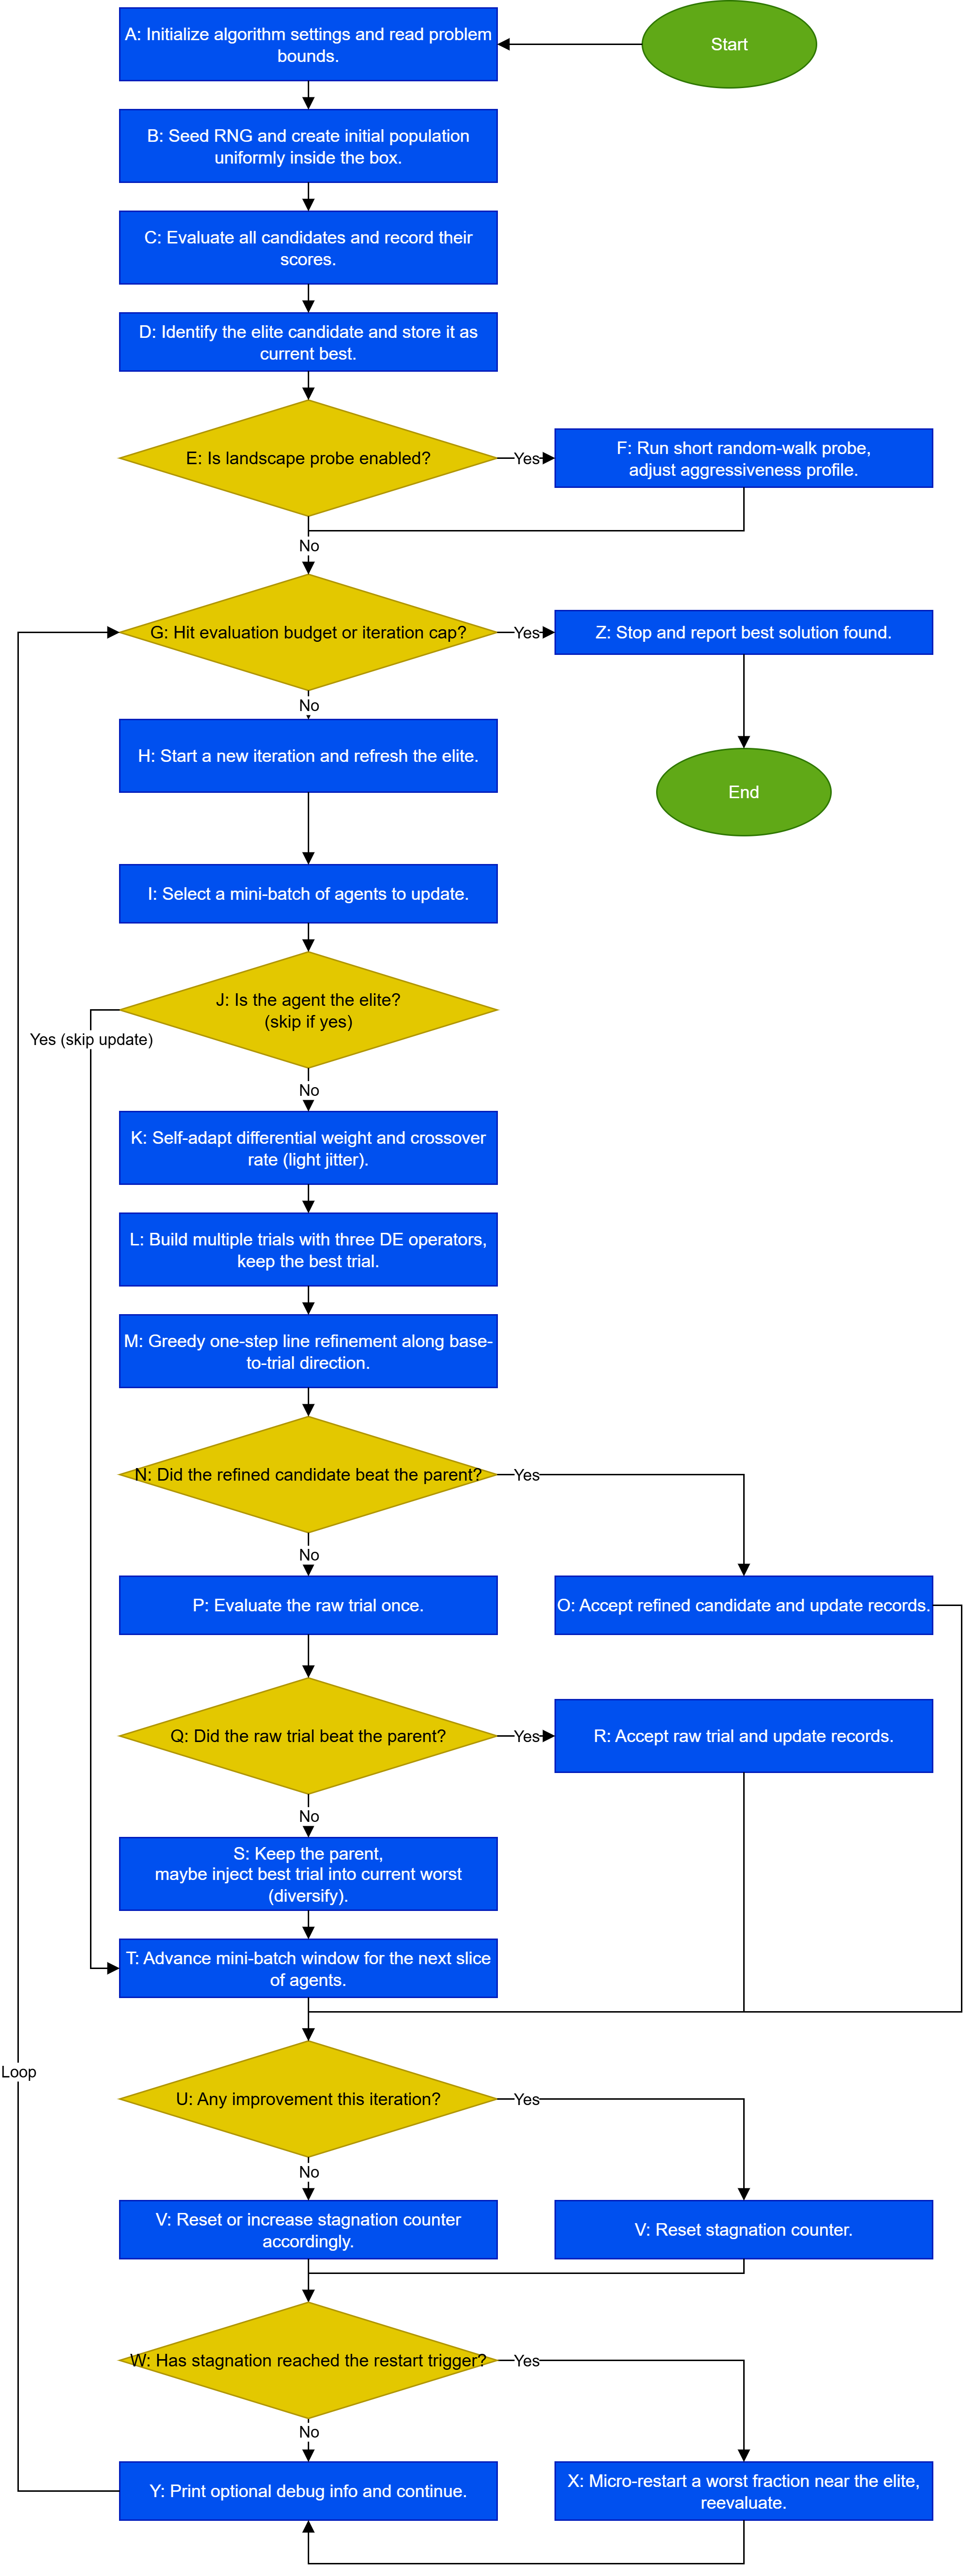
\includegraphics[scale=0.5]{tridentde_flow}

\caption{TRIDENT-DE flowchart: triple-operator DE with greedy refinement and
adaptive micro-restarts\protect\label{fig:flowchart}}
\end{figure}

As shown in Figure \ref{fig:flowchart}, after initialization and
elite refresh, each agent undergoes operator selection, parameter
jitter, trial construction, and greedy line refinement, followed if
necessary by a single raw-trial evaluation. Iteration-level progress
is assessed at node U, to avoid ambiguity, the “Yes” and “No” branches
lead to separate actions V (reset stagnation counter) and Y (increase
stagnation counter) which both feed into W (restart trigger). When
the trigger fires, micro-restarts (X) rejuvenate a worst fraction
near the elite (or uniformly), after which the loop returns to the
main termination check. This organization clarifies control flow,
emphasizes the low-cost refinement step, and shows precisely how stagnation
governs diversity injection.

\section{Experimental setup and benchmark results\protect\label{sec:Results}}

\subsection{Setup\protect\label{subsec:Setup}}

Table \ref{tab:parameters} summarizes the core settings of TRIDENT-DE,
grouping the population size, the box bounds, and the default DE controls
($F$, $C$) together with the jDE-style self-adaptation (resampling
probabilities and sampling ranges). It also lists the hyperparameters
governing the triple trial-vector ensemble, the greedy line-refinement,
and the adaptive micro-restart policy (restart fraction $\rho$, Gaussian
kick scale $\sigma$, stagnation trigger $\tau$). Note that operator
scheduling follows a round-robin (three operators) scheme in the manuscript,
while the implementation uses a round-robin (three operators) to balance
exploration and exploitation across iterations. The defaults $\mathrm{FE}_{\max}$
= $1.5\cdot10^{5}$ and $I_{\max}$ = 500 standardize the computational
budget across problems and act as termination criteria, with priority
given to the evaluation budget (see Table \ref{tab:parameters})

\begin{table}[H]
\centering{}\caption{TRIDENT-DE parameters\protect\label{tab:parameters}}
\begin{tabular}{ccl}
\hline 
{\footnotesize\textbf{Name}} & {\footnotesize\textbf{Value}} & {\footnotesize\textbf{Description}}\tabularnewline
\hline 
{\footnotesize$N$} & {\footnotesize 100} & {\footnotesize Population size}\tabularnewline
\hline 
{\footnotesize$n$} & {\footnotesize problem} & {\footnotesize Problem dimension (from instance).}\tabularnewline
\hline 
{\footnotesize$[\ell,u]$} & {\footnotesize from problem, fallback $[-1,1]^{n}$} & {\footnotesize Box bounds, fallback used if margins missing.}\tabularnewline
\hline 
{\footnotesize$F$} & {\footnotesize$F^{0}=0.9$} & {\footnotesize Baseline scale, per-individual $F_{i}$ (jDE-style control
in code).}\tabularnewline
\hline 
{\footnotesize$C$} & {\footnotesize$C^{0}=0.7$} & {\footnotesize Baseline crossover, per-individual $C_{i}$ (jDE-style
control in code).}\tabularnewline
\hline 
{\footnotesize$r,q,p$} & {\footnotesize (round-robin)} & {\footnotesize Operator selection in manuscript, implementation uses
3-operator cycle.}\tabularnewline
\hline 
{\footnotesize$\tau$} & {\footnotesize 18} & {\footnotesize Stagnation trigger (no-improvement iterations before
restart).}\tabularnewline
\hline 
{\footnotesize$\rho$} & {\footnotesize 0.10} & {\footnotesize Fraction of worst individuals to restart.}\tabularnewline
\hline 
{\footnotesize$\sigma$} & {\footnotesize 0.20} & {\footnotesize Gaussian kick scale at restart ($\times$ box range).}\tabularnewline
\hline 
{\footnotesize$\beta$} & {\footnotesize$\{1.0,\,0.5\}$} & {\footnotesize One-step greedy line-refine factors.}\tabularnewline
\hline 
{\footnotesize$\mathrm{FE}_{\max}$} & {\footnotesize 150,000} & {\footnotesize Evaluation-budget termination (code default).}\tabularnewline
\hline 
{\footnotesize$I_{\max}$} & {\footnotesize 500} & {\footnotesize Iteration cap (used in manuscript, not enforced by code).}\tabularnewline
\hline 
{\footnotesize$\alpha$} & {\footnotesize 0.55} & {\footnotesize Mini-batch ratio.}\tabularnewline
\hline 
{\footnotesize$t$} & {\footnotesize 4} & {\footnotesize Trials per agent.}\tabularnewline
\hline 
{\footnotesize$\tau_{F}$} & {\footnotesize 0.10} & {\footnotesize jDE resampling prob. for $F_{i}$.}\tabularnewline
\hline 
{\footnotesize$\tau_{C}$} & {\footnotesize 0.10} & {\footnotesize jDE resampling prob. for $C_{i}$.}\tabularnewline
\hline 
{\footnotesize$F_{\ell},F_{u}$} & {\footnotesize$0.1,\,1.2$} & {\footnotesize Bounds for jDE resampling of $F_{i}$.}\tabularnewline
\hline 
{\footnotesize$C_{\ell},C_{u}$} & {\footnotesize$0.0,\,0.95$} & {\footnotesize Bounds for jDE resampling of $C_{i}$.}\tabularnewline
\hline 
{\footnotesize$\varphi$} & {\footnotesize 0.10} & {\footnotesize Top-$p$ fraction for pbest/1.}\tabularnewline
\hline 
\end{tabular}
\end{table}

Table \ref{tab:parametes2} reports the configurations of all competitor
methods to ensure reproducibility and fairness with respect to population
size and iteration budget. For each algorithm, we list its internal
controls (e.g., the comprehensive-learning probability for CLPSO,
population sizing and coefficients for CMA-ES, JADE-style parameters
for EA4Eig, success-history memories and p-best ranges for mLSHADE\_RL
and UDE3, and adaptation schemes for SaDE) as used in our experiments.
Harmonizing the population at $N$ = 100 and the iteration cap at
$I_{\max}$ = 500 guarantees comparability, while per-method settings
follow the literature and publicly available implementations. 
\begin{table}[H]
\caption{Parameters of other methods\protect\label{tab:parametes2}}

\centering{}%
\begin{tabular}{ccc}
\hline 
\textbf{Name} & \textbf{Value} & \textbf{Description}\tabularnewline
\hline 
\hline 
$N$ & 100 & Population size for all methods\tabularnewline
\hline 
$I_{\max}$ & 500 & Maximum number of iterations for all methods\tabularnewline
\hline 
\multicolumn{3}{c}{\textbf{CLPSO}}\tabularnewline
\hline 
clProb & 0.3 & Comprehensive learning probability\tabularnewline
\hline 
cognitiveWeight & 1.49445 & Cognitive weight\tabularnewline
\hline 
inertiaWeight & 0.729 & Inertia weight\tabularnewline
\hline 
mutationRate & 0.01 & Mutation rate\tabularnewline
\hline 
socialWeight & 1.49445 & Social weight\tabularnewline
\hline 
\multicolumn{3}{c}{\textbf{CMA-ES}}\tabularnewline
\hline 
$N_{CMA-ES}$ & $4+\left\lfloor 3\cdot\log(dim)\right\rfloor $ & Population size\tabularnewline
\hline 
\multicolumn{3}{c}{\textbf{EA4Eig}}\tabularnewline
\hline 
archiveSize & 100 & Archive size for JADE-style mutation\tabularnewline
\hline 
eig\_interval & 5 & Recompute eigenbasis every k iterations\tabularnewline
\hline 
maxCR & 1 & Upper bound for CR\tabularnewline
\hline 
maxF & 1 & Upper bound for F\tabularnewline
\hline 
minCR & 0 & Lower bound for CR\tabularnewline
\hline 
minF & 0.1 & Lower bound for F\tabularnewline
\hline 
pbest & 0.2 & p-best fraction (current-to-pbest/1)\tabularnewline
\hline 
tauCR & 0.1 & Self-adaptation prob. for CR\tabularnewline
\hline 
tauF & 0.1 & Self-adaptation prob. for F\tabularnewline
\hline 
\multicolumn{3}{c}{\textbf{mLSHADE\_RL}}\tabularnewline
\hline 
archiveSize & 500 & Archive size\tabularnewline
\hline 
memorySize & 10 & Success-history memory size (H)\tabularnewline
\hline 
minPopulation & 4 & Minimum population size\tabularnewline
\hline 
pmax & 0.2 & Maximum p-best fraction\tabularnewline
\hline 
pmin & 0.05 & Minimum p-best fraction\tabularnewline
\hline 
\multicolumn{3}{c}{\textbf{SaDE}}\tabularnewline
\hline 
crSigma & 0.1 & Std for CR sampling\tabularnewline
\hline 
fGamma & 0.1 & Scale for Cauchy F sampling\tabularnewline
\hline 
initCR & 0.5 & Initial CR mean\tabularnewline
\hline 
initF & 0.7 & Initial F mean\tabularnewline
\hline 
learningPeriod & 25 & Iterations per adaptation window\tabularnewline
\hline 
\multicolumn{3}{c}{\textbf{UDE3}}\tabularnewline
\hline 
minPopulation & 4 & Minimum population size.\tabularnewline
\hline 
memorySize & 10 & Success-history memory size (H).\tabularnewline
\hline 
archiveSize & 100 & Archive size.\tabularnewline
\hline 
pmin & 0.05 & Minimum p-best fraction.\tabularnewline
\hline 
pmax & 0.2 & Maximum p-best fraction.\tabularnewline
\hline 
\end{tabular}
\end{table}

All experiments were conducted on a high-performance node featuring
an AMD Ryzen 9 5950X CPU (16 cores, 32 threads) and 128 GB of DDR4
memory, running Debian Linux. The evaluation protocol was designed
for statistical rigor and reproducibility: each benchmark function
was executed 30 times independently, using distinct random seeds to
capture the stochastic variability of the algorithms.

The proposed method and all baselines were implemented in optimized
ANSI C++ and integrated into the open-source OPTIMUS framework \citep{optimus}.
The source code is hosted at \url{https://github.com/itsoulos/GLOBALOPTIMUS}
(accessed September 25, 2025), ensuring transparency and reproducibility.
Parameter settings exactly follow Tables \ref{tab:parameters} and
\ref{tab:parametes2}. Build environment: Debian 12.12 with GCC 13.4.

The primary performance indicator is the average number of objective-function
evaluations over 30 runs for each test function. In all ranking tables
comparing solvers, best values are highlighted in green (1st place)
and second-best values in blue (2nd place).

\subsection{Benchmark functions\protect\label{subsec:BenchmarFunctions}}

Table \ref{tab:benchmarkFunctions} compiles the real-world optimization
problems used in our evaluation. For each case, we report a brief
description, the dimensionality and variable types (continuous/mixed-integer),
the nature and count of constraints (inequalities/equalities), salient
landscape properties (nonconvexity, multi-modality), as well as the
evaluation budget and comparison criteria. The set spans, indicatively,
mechanical design, energy scheduling, process optimization, and parameter
estimation with black-box simulators, ensuring that conclusions extend
beyond synthetic test functions. Where applicable, we also note any
normalizations or constraint reformulations adopted for fair comparison.

\begin{table}[H]
\caption{The real world benchmark functions used in the conducted experiments
\protect\label{tab:benchmarkFunctions}}

\centering{}{\tiny{}%
\begin{tabular}{cccc}
\hline 
{\scriptsize\textbf{Problem}} & {\scriptsize\textbf{Formula}} & {\scriptsize\textbf{Dim}} & {\scriptsize\textbf{Constraints/Bounds}}\tabularnewline
\hline 
\hline 
\begin{cellvarwidth}[m]
\centering
{\tiny\textbf{Parameter}}{\tiny\par}

{\tiny\textbf{Estimation for}}{\tiny\par}

{\tiny\textbf{Frequency-Modulated}}{\tiny\par}

{\tiny\textbf{Sound Waves}}
\end{cellvarwidth} & \begin{cellvarwidth}[m]
\centering
{\tiny$\min_{x\in[-6.4,6.35]^{6}}\;f(x)=\frac{1}{N}\sum_{n=1}^{N}\left|y(n;x)-y_{\text{target}}(n)\right|^{2}$}{\tiny\par}

{\tiny$y(n;x)=x_{0}\sin\left(x_{1}n+x_{2}\sin(x_{3}n+x_{4}\sin(x_{5}n))\right)$}
\end{cellvarwidth} & {\tiny 6} & {\tiny$x_{i}\in[-6.4,6.35]$}\tabularnewline
\hline 
\begin{cellvarwidth}[m]
\centering
{\tiny\textbf{Lennard-Jones}}{\tiny\par}

{\tiny\textbf{Potential}}{\tiny\par}

{\tiny\textbf{(atoms: 10, 13, 38)}}
\end{cellvarwidth} & {\tiny$\min_{x\in\mathbb{R}^{3N-6}}\;f(x)=4\sum_{i=1}^{N-1}\sum_{j=i+1}^{N}\left[\left(\frac{1}{r_{ij}}\right)^{12}-\left(\frac{1}{r_{ij}}\right)^{6}\right]$} & \begin{cellvarwidth}[m]
\centering
{\tiny 24,}{\tiny\par}

{\tiny 43,}{\tiny\par}

{\tiny 108}
\end{cellvarwidth} & \begin{cellvarwidth}[m]
\centering
{\tiny$x_{0}\in(0,0,0)$}{\tiny\par}

{\tiny$x_{1},x_{2}\in[0,4]$}{\tiny\par}

{\tiny$x_{3}\in[0,\pi]$}{\tiny\par}

{\tiny$x_{3k-3}$}{\tiny\par}

{\tiny$x_{3k-2}$}{\tiny\par}

{\tiny$x_{i}\in[-b_{k},+b_{k}]$}
\end{cellvarwidth}\tabularnewline
\hline 
\begin{cellvarwidth}[m]
\centering
{\tiny\textbf{Bifunctional Catalyst}}{\tiny\par}

{\tiny\textbf{Blend Optimal Control}}
\end{cellvarwidth} & \begin{cellvarwidth}[m]
\centering
{\tiny$\frac{dx_{1}}{dt}=-k_{1}x_{1}$, $\frac{dx_{2}}{dt}=k_{1}x_{1}-k_{2}x_{2}+k_{3}x_{2}+k_{4}x_{3}$,}{\tiny\par}

{\tiny$\frac{dx_{3}}{dt}=k_{2}x_{2}$, $\frac{dx_{4}}{dt}=-k_{4}x_{4}+k_{5}x_{5}$,}{\tiny\par}

{\tiny$\frac{dx_{5}}{dt}=-k_{3}x_{2}+k_{6}x_{4}-k_{5}x_{5}+k_{7}x_{6}+k_{8}x_{7}+k_{9}x_{5}+k_{10}x_{7}$}{\tiny\par}

{\tiny$\frac{dx_{6}}{dt}=k_{8}x_{5}-k_{7}x_{6}$, $\frac{dx_{7}}{dt}=k_{9}x_{5}-k_{10}x_{7}$}{\tiny\par}

{\tiny$k_{i}(u)=c_{i1}+c_{i2}u+c_{i3}u^{2}+c_{i4}u^{3}$}
\end{cellvarwidth} & {\tiny 1} & {\tiny$u\in[0.6,0.9]$}\tabularnewline
\hline 
\begin{cellvarwidth}[m]
\centering
{\tiny\textbf{Optimal Control of a}}{\tiny\par}

{\tiny\textbf{Non-Linear Stirred}}{\tiny\par}

{\tiny\textbf{Tank Reactor}}
\end{cellvarwidth} & \begin{cellvarwidth}[m]
\centering
{\tiny$J(u)=\int_{0}^{0.72}\left[x_{1}(t)^{2}+x_{2}(t)^{2}+0.1u^{2}\right]dt$}{\tiny\par}

{\tiny$\frac{dx_{1}}{dt}=-2x_{1}+x_{2}+1.25u+0.5\exp\left(\frac{x_{1}}{x_{1}+2}\right)$}{\tiny\par}

{\tiny$\frac{dx_{2}}{dt}=-x_{2}+0.5\exp\left(\frac{x_{1}}{x_{1}+2}\right)$}{\tiny\par}

{\tiny$x_{1}(0)=0.9,\quad x_{2}(0)=0.09$, $t\in[0,0.72]$}
\end{cellvarwidth} & {\tiny 1} & {\tiny$u\in[0,5]$}\tabularnewline
\hline 
\begin{cellvarwidth}[m]
\centering
{\tiny\textbf{Tersoff Potential}}{\tiny\par}

{\tiny\textbf{for model Si (B)}}
\end{cellvarwidth} & \begin{cellvarwidth}[m]
\centering
{\tiny$\min_{\mathbf{x}\in\Omega}f(\mathbf{x})=\sum_{i=1}^{N}E(\mathbf{x}_{i})$}{\tiny\par}

{\tiny$E(\mathbf{x}_{i})=\frac{1}{2}\sum_{j\neq i}f_{c}(r_{ij})\left[V_{R}(r_{ij})-B_{ij}V_{A}(r_{ij})\right]$}{\tiny\par}

{\tiny where $r_{ij}=\|\mathbf{x}_{i}-\mathbf{x}_{j}\|$, $V_{R}(r)=A\exp(-\lambda_{1}r)$}{\tiny\par}

{\tiny$V_{A}(r)=B\exp(-\lambda_{2}r)$}{\tiny\par}

{\tiny$f_{c}(r)$: cutoff function with $f_{c}(r)$: angle parameter}
\end{cellvarwidth} & {\tiny 30} & \begin{cellvarwidth}[m]
\centering
{\tiny$x_{1}\in[0,4]$}{\tiny\par}

{\tiny$x_{2}\in[0,4]$}{\tiny\par}

{\tiny$x_{3}\in[0,\pi]$}{\tiny\par}

{\tiny$x_{i}\in\left[\frac{4(i-3)}{4},\ 4\right]$}
\end{cellvarwidth}\tabularnewline
\hline 
\begin{cellvarwidth}[m]
\centering
{\tiny\textbf{Tersoff Potential}}{\tiny\par}

{\tiny\textbf{for model Si (C)}}
\end{cellvarwidth} & \begin{cellvarwidth}[m]
\centering
{\tiny$\min_{\mathbf{x}}\;V(\mathbf{x})=\sum_{i=1}^{N}\sum_{j>i}^{N}f_{C}(r_{ij})\left[a_{ij}f_{R}(r_{ij})+b_{ij}f_{A}(r_{ij})\right]$}{\tiny\par}

{\tiny$f_{C}(r)=\begin{cases}
1, & r<R-D\\
\frac{1}{2}+\frac{1}{2}\cos\left(\frac{\pi(r-R+D)}{2D}\right), & |r-R|\leq D\\
0, & r>R+D
\end{cases}$}{\tiny\par}

{\tiny$f_{R}(r)=A\exp(-\lambda_{1}r)$}{\tiny\par}

{\tiny$f_{A}(r)=-B\exp(-\lambda_{2}r)$}{\tiny\par}

{\tiny$b_{ij}=\left[1+(\beta^{n})\zeta_{ij}^{n}\right]^{-1/(2n)}$}{\tiny\par}

{\tiny$\sum_{k\neq i,j}f_{C}(r_{ik})g(\theta_{ijk})\exp\left[\lambda_{3}^{3}(r_{ij}-r_{ik})^{3}\right]$}
\end{cellvarwidth} & {\tiny 30} & \begin{cellvarwidth}[m]
\centering
{\tiny$x_{1}\in[0,4]$}{\tiny\par}

{\tiny$x_{2}\in[0,4]$}{\tiny\par}

{\tiny$x_{3}\in[0,\pi]$}{\tiny\par}

{\tiny$x_{i}\in\left[\frac{4(i-3)}{4},\ 4\right]$}
\end{cellvarwidth}\tabularnewline
\hline 
\begin{cellvarwidth}[m]
\centering
{\tiny\textbf{Spread}}{\tiny\par}

{\tiny\textbf{Spectrum Radar}}{\tiny\par}

{\tiny\textbf{Polyphase}}{\tiny\par}

{\tiny\textbf{Code Design}}
\end{cellvarwidth} & \begin{cellvarwidth}[m]
\centering
{\tiny$\min_{x\in X}\;f(x)=\max\left\{ |\varphi_{1}(x)|,|\varphi_{2}(x)|,\ldots,|\varphi_{m}(x)|\right\} $}{\tiny\par}

{\tiny$X=\{x\in\mathbb{R}^{n}\mid0\leq x_{j}\leq2\pi,\;j=1,\ldots,n\}m=2n-1$}{\tiny\par}

{\tiny$\varphi_{j}(x)=\begin{cases}
{\displaystyle \sum_{k=1}^{n-j}\cos(x_{k}-x_{k+j})} & \text{for }j=1,\ldots,n-1\\
{\displaystyle n} & \text{for }j=n\\
{\displaystyle \varphi_{2n-j}(x)} & \text{for }j=n+1,\ldots,2n-1
\end{cases}$}{\tiny\par}

{\tiny$\varphi_{j}(x)=\sum_{k=1}^{n-j}\cos(x_{k}-x_{k+j}),\quad j=1,\ldots,n-1$}{\tiny\par}

{\tiny$\varphi_{n}(x)=n$, $\varphi_{n+\ell}(x)=\varphi_{n-\ell}(x),\quad\ell=1,\ldots,n-1$}
\end{cellvarwidth} & {\tiny 20} & {\tiny$x_{j}\in[0,2\pi]$}\tabularnewline
\hline 
\begin{cellvarwidth}[m]
\centering
{\tiny\textbf{Transmission Network}}{\tiny\par}

{\tiny\textbf{Expansion Planning}}
\end{cellvarwidth} & \begin{cellvarwidth}[m]
\centering
{\tiny$\min\sum_{l\in\Omega}c_{l}n_{l}+W_{1}\sum_{l\in OL}|f_{l}-\bar{f}_{l}|+W_{2}\sum_{l\in\Omega}\max(0,n_{l}-\bar{n}_{l})$}{\tiny\par}

{\tiny$Sf=g-d$}{\tiny\par}

{\tiny$f_{l}=\gamma_{l}n_{l}\Delta\theta_{l},\quad\forall l\in\Omega$}{\tiny\par}

{\tiny$|f_{l}|\leq\bar{f}_{l}n_{l},\quad\forall l\in\Omega$}{\tiny\par}

{\tiny$0\leq n_{l}\leq\bar{n}_{l},\quad n_{l}\in\mathbb{Z},\quad\forall l\in\Omega$}
\end{cellvarwidth} & {\tiny 7} & \begin{cellvarwidth}[m]
\centering
{\tiny$0\leq n_{i}\leq\bar{n}_{l}$}{\tiny\par}

{\tiny$n_{i}\in\mathbb{Z}$}
\end{cellvarwidth}\tabularnewline
\hline 
\begin{cellvarwidth}[m]
\centering
{\tiny\textbf{Electricity}}{\tiny\par}

{\tiny\textbf{Transmission}}{\tiny\par}

{\tiny\textbf{Pricing}}
\end{cellvarwidth} & \begin{cellvarwidth}[m]
\centering
{\tiny$\min_{x}\;\;f(x)=\sum_{i=1}^{N_{g}}\left(\frac{C_{i}^{gen}}{P_{i}^{gen}}-R_{i}^{gen}\right)^{2}+\sum_{j=1}^{N_{d}}\left(\frac{C_{j}^{load}}{P_{j}^{load}}-R_{j}^{load}\right)^{2}$}{\tiny\par}

{\tiny$\sum_{j}GD_{i,j}+\sum_{j}BT_{i,j}=P_{i}^{gen},\quad\forall i$}{\tiny\par}

{\tiny$\sum_{i}GD_{i,j}+\sum_{i}BT_{i,j}=P_{j}^{load},\quad\forall j$}{\tiny\par}

{\tiny$GD_{i,j}^{max}=\min(P_{i}^{gen}-BT_{i,j},\;P_{j}^{load}-BT_{i,j})$}
\end{cellvarwidth} & {\tiny 126} & {\tiny$GD_{i,j}\in[0,GD_{i,j}^{max}]$}\tabularnewline
\hline 
\begin{cellvarwidth}[m]
\centering
{\tiny\textbf{Circular Antenna}}{\tiny\par}

{\tiny\textbf{Array Design}}
\end{cellvarwidth} & \begin{cellvarwidth}[m]
\centering
{\tiny$\min_{r_{1},\ldots,r_{6},\,\varphi_{1},\ldots,\varphi_{6}}\quad f(\mathbf{x})=\max_{\theta\in\Omega}AF(\mathbf{x},\theta)$}{\tiny\par}

{\tiny$AF(\mathbf{x},\theta)=\left|\sum_{k=1}^{6}\exp\left(j\left[2\pi r_{k}\cos(\theta-\theta_{k})+\varphi_{k}\frac{\pi}{180}\right]\right)\right|$}
\end{cellvarwidth} & {\tiny 12} & \begin{cellvarwidth}[m]
\centering
{\tiny$r_{k}\in[0.2,1]$}{\tiny\par}

{\tiny$\varphi_{k}\in[-180,180]$}
\end{cellvarwidth}\tabularnewline
\hline 
\begin{cellvarwidth}[m]
\centering
{\tiny\textbf{Cassini 2:}}{\tiny\par}

{\tiny\textbf{Spacecraft Trajectory}}{\tiny\par}

{\tiny\textbf{Optimization Problem}}
\end{cellvarwidth} & \begin{cellvarwidth}[m]
\centering
{\tiny$x=\big[t_{0},\;\Delta t_{1},\ldots,\Delta t_{5},\;p_{1},\ldots,p_{4}\big]^{\top},$}{\tiny\par}

{\tiny$\min_{x}J(x)=\Delta v_{\text{launch}}+\sum_{\ell=1}^{4}\Delta v_{\ell}^{\text{DSM}}+\Delta v_{\text{arrival}},$}{\tiny\par}

{\tiny$E\;\rightarrow\;V\;\rightarrow\;E\;\rightarrow\;V\;\rightarrow\;J\;\rightarrow\;S$}{\tiny\par}

{\tiny$t_{0}\in[850,\;2000],\qquad\Delta t_{\ell}\in[20,\;1200],\qquad p_{\ell}\in[1.0,\;10.0].$}
\end{cellvarwidth} & {\tiny 10} & \begin{cellvarwidth}[m]
\centering
{\tiny$r_{p,\ell}\ge R_{P_{\ell}}+h_{\min,P_{\ell}},$}{\tiny\par}

{\tiny$\delta_{\ell}\le\delta_{\max,P_{\ell}},$}{\tiny\par}

{\tiny$t_{0}^{\min}\le t_{0}\le t_{0}^{\max},$}{\tiny\par}

{\tiny$\Delta t_{\ell}^{\min}\le\Delta t_{\ell}\le\Delta t_{\ell}^{\max}.$}
\end{cellvarwidth}\tabularnewline
\hline 
\begin{cellvarwidth}[m]
\centering
{\tiny\textbf{Wireless Coverage}}{\tiny\par}

{\tiny\textbf{Antenna Placement}}
\end{cellvarwidth} & \begin{cellvarwidth}[m]
\centering
{\tiny$x_{i},\ y_{i}\in\mathbb{R}\quad(\text{position}),P_{i}\in\mathbb{R}_{\ge0}\quad(\text{transmission power}).$}{\tiny\par}

{\tiny$S_{iu}(x_{i},y_{i},P_{i})\;=\;\frac{G\,P_{i}}{\bigl(\,(x_{i}-x_{u})^{2}+(y_{i}-y_{u})^{2}\,\bigr)^{\alpha/2}+\varepsilon},$}{\tiny\par}

{\tiny$\min_{x,y,P}\;\underbrace{\sum_{u\in\mathcal{U}}\bigl[\tau-S_{u}(x,P)\bigr]_{+}}_{\text{coverage deficiency}}\;+\;\lambda_{P}\sum_{i=1}^{N}P_{i}\;+,$}{\tiny\par}

{\tiny$\;\lambda_{O}\sum_{u\in\mathcal{U}}\sum_{i<j}\bigl[\min\{S_{iu},S_{ju}\}-\kappa\bigr]_{+}$}{\tiny\par}

{\tiny$S_{u}(x,P)\;=\;\max_{i=1,\dots,N}\,S_{iu}(x_{i},y_{i},P_{i}).$}
\end{cellvarwidth} & {\tiny 30} & \begin{cellvarwidth}[m]
\centering
{\tiny$0\le x_{i}\le W,$}{\tiny\par}

{\tiny$0\le y_{i}\le H,$}{\tiny\par}

{\tiny$0\le P_{i}\le P_{\max}$}
\end{cellvarwidth}\tabularnewline
\hline 
\begin{cellvarwidth}[m]
\centering
{\tiny\textbf{Dynamic}}{\tiny\par}

{\tiny\textbf{Economic}}{\tiny\par}

{\tiny\textbf{Dispatch 1}}
\end{cellvarwidth} & \begin{cellvarwidth}[m]
\centering
{\tiny$\min_{\mathbf{P}}\quad f(\mathbf{P})=\sum_{t=1}^{24}\sum_{i=1}^{5}\left(a_{i}P_{i,t}^{2}+b_{i}P_{i,t}+c_{i}\right)$}{\tiny\par}

{\tiny$P_{i}^{\min}\leq P_{i,t}\leq P_{i}^{\max},\quad\forall i=1,\ldots,5,\;t=1,\ldots,24$}{\tiny\par}

{\tiny$\sum_{i=1}^{5}P_{i,t}=D_{t},\quad\forall t=1,\ldots,24$}{\tiny\par}

{\tiny$P_{\min}=[10,20,30,40,50]$}{\tiny\par}

{\tiny$P_{\max}=[75,125,175,250,300]$}
\end{cellvarwidth} & {\tiny 120} & {\tiny$P_{i}^{\min}\leq P_{i,t}\leq P_{i}^{\max}$}\tabularnewline
\hline 
\begin{cellvarwidth}[m]
\centering
{\tiny\textbf{Dynamic}}{\tiny\par}

{\tiny\textbf{Economic}}{\tiny\par}

{\tiny\textbf{Dispatch 2}}
\end{cellvarwidth} & \begin{cellvarwidth}[m]
\centering
{\tiny$\min_{\mathbf{P}}\quad f(\mathbf{P})=\sum_{t=1}^{24}\sum_{i=1}^{9}\left(a_{i}P_{i,t}^{2}+b_{i}P_{i,t}+c_{i}\right)$}{\tiny\par}

{\tiny$P_{i}^{\min}\leq P_{i,t}\leq P_{i}^{\max},\quad\forall i=1,\ldots,5,\;t=1,\ldots,24$}{\tiny\par}

{\tiny$\sum_{i=1}^{5}P_{i,t}=D_{t},\quad\forall t=1,\ldots,24$}{\tiny\par}

{\tiny$P_{\min}=[150,135,73,60,73,57,20,47,20]$}{\tiny\par}

{\tiny$P_{\max}=[470,460,340,300,243,160,130,120,80]$}
\end{cellvarwidth} & {\tiny 216} & {\tiny$P_{i}^{\min}\leq P_{i,t}\leq P_{i}^{\max}$}\tabularnewline
\hline 
\begin{cellvarwidth}[m]
\centering
{\tiny\textbf{Static}}{\tiny\par}

{\tiny\textbf{Economic}}{\tiny\par}

{\tiny\textbf{Load}}{\tiny\par}

{\tiny\textbf{Dispatch}}{\tiny\par}

{\tiny\textbf{(1,2,3,4,5)}}
\end{cellvarwidth} & \begin{cellvarwidth}[m]
\centering
{\tiny$\min_{P_{1},\ldots,P_{N_{G}}}F=\sum_{i=1}^{N_{G}}f_{i}(P_{i})$}{\tiny\par}

{\tiny$f_{i}(P_{i})=a_{i}P_{i}^{2}+b_{i}P_{i}+c_{i},\quad i=1,2,\ldots,N_{G}$}{\tiny\par}

{\tiny$f_{i}(P_{i})=a_{i}P_{i}^{2}+b_{i}P_{i}+c_{i}+|e_{i}\sin(f_{i}(P_{i}^{\min}-P_{i}))|$}{\tiny\par}

{\tiny$P_{i}^{\min}\leq P_{i}\leq P_{i}^{\max},\quad i=1,2,\ldots,N_{G}$}{\tiny\par}

{\tiny$\sum_{i=1}^{N_{G}}P_{i}=P_{D}+P_{L}$}{\tiny\par}

{\tiny$P_{L}=\sum_{i=1}^{N_{G}}\sum_{j=1}^{N_{G}}P_{i}B_{ij}P_{j}+\sum_{i=1}^{N_{G}}B_{0i}P_{i}+B_{00}$}{\tiny\par}

{\tiny$P_{i}-P_{i}^{0}\leq UR_{i}\quad P_{i}^{0}-P_{i}\leq DR_{i}$}
\end{cellvarwidth} & \begin{cellvarwidth}[m]
\centering
{\tiny 6}{\tiny\par}

{\tiny 13}{\tiny\par}

{\tiny 15}{\tiny\par}

{\tiny 40}{\tiny\par}

{\tiny 140}
\end{cellvarwidth} & \begin{cellvarwidth}[m]
\centering
{\tiny See}{\tiny\par}

{\tiny Technical}{\tiny\par}

{\tiny Report}{\tiny\par}

{\tiny of}{\tiny\par}

{\tiny CEC2011}
\end{cellvarwidth}\tabularnewline
\hline 
\end{tabular}}{\tiny\par}
\end{table}


\subsection{Parameter sensitivity analysis of TRIDENT-DE\protect\label{subsec:sensitivity}}

Following Lee et al.’s \citep{Lee} parameter-sensitivity methodology,
we construct a structured analysis to quantify responsiveness to parameter
changes and the preservation of reliability across diverse operating
regimes.

\begin{table}[H]
\caption{Sensitivity analysis of the method parameters for the ``Lennard-Jones
Potential, Dim:10'' problem\protect\label{tab:lennard}}

\centering{}%
\begin{tabular}{ccccccc}
\hline 
\textbf{Parameter} & \textbf{Value} & \textbf{Mean} & \textbf{Min} & \textbf{Max} & \textbf{Iters} & \textbf{Main effect range}\tabularnewline
\hline 
\hline 
\multirow{3}{*}{$\tau$} & 12 & -27.0878 & -28.4225 & -24.0293 & 3240 & \multirow{3}{*}{0.0137}\tabularnewline
\cline{2-6}
 & 18 & -27.0741 & -28.4225 & -23.2567 & 3240 & \tabularnewline
\cline{2-6}
 & 30 & -27.0871 & -28.4225 & -23.0968 & 3240 & \tabularnewline
\hline 
\multirow{3}{*}{$\rho$} & 0.05 & -27.0741 & -28.4225 & -23.0968 & 3240 & \multirow{3}{*}{0.0143}\tabularnewline
\cline{2-6}
 & 0.1 & -27.0885 & -28.4225 & -23.1044 & 3240 & \tabularnewline
\cline{2-6}
 & 0.2 & -27.0864 & -28.4225 & -23.6869 & 3240 & \tabularnewline
\hline 
\multirow{3}{*}{$\sigma$} & 0.1 & -27.0913 & -28.4225 & -23.6906 & 3240 & \multirow{3}{*}{0.0138}\tabularnewline
\cline{2-6}
 & 0.2 & -27.0803 & -28.4225 & -23.1044 & 3240 & \tabularnewline
\cline{2-6}
 & 0.3 & -27.0775 & -28.4225 & -23.0968 & 3240 & \tabularnewline
\hline 
\multirow{4}{*}{$t$} & 2 & -27.0823 & -28.4225 & -23.1044 & 3240 & \multirow{4}{*}{0.0066}\tabularnewline
\cline{2-6}
 & 4 & -27.0861 & -28.4225 & -23.2567 & 3240 & \tabularnewline
\cline{2-6}
 & 6 & -27.0842 & -28.4225 & -23.0968 & 3240 & \tabularnewline
\cline{2-6}
 & 8 & -27.0794 & -28.4225 & -23.6906 & 3240 & \tabularnewline
\hline 
\multirow{3}{*}{$\varphi$} & 0.06 & -27.0916 & -28.4225 & -23.0968 & 3240 & \multirow{3}{*}{0.0145}\tabularnewline
\cline{2-6}
 & 0.1 & -27.0803 & -28.4225 & -23.2567 & 3240 & \tabularnewline
\cline{2-6}
 & 0.18 & -27.0771 & -28.4225 & -23.1044 & 3240 & \tabularnewline
\hline 
\end{tabular}
\end{table}
\begin{figure}[H]
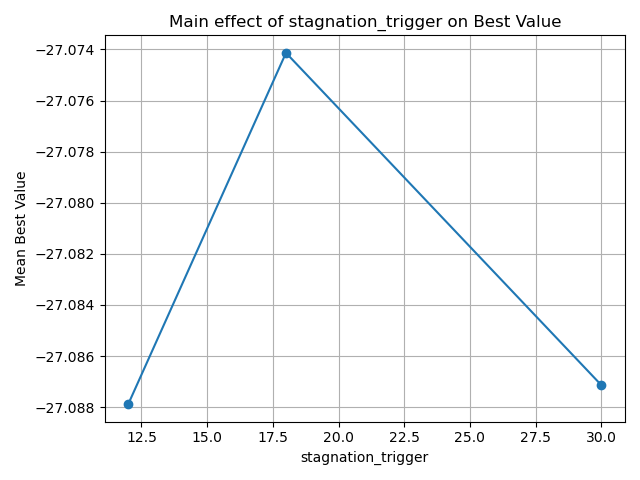
\includegraphics[scale=0.25]{potential10_stagnationTrigger}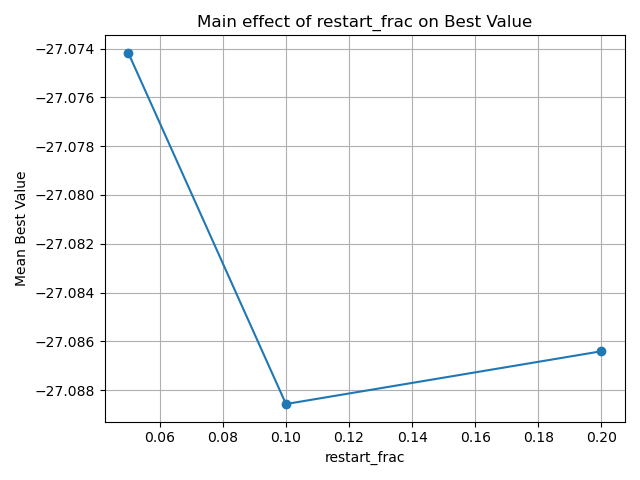
\includegraphics[scale=0.25]{potential10_restartFrac}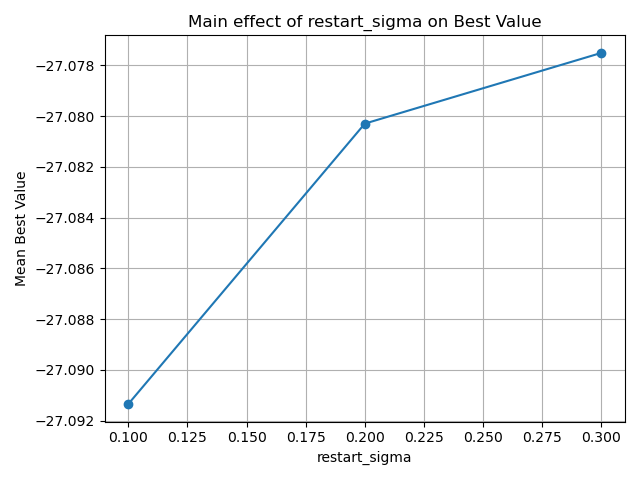
\includegraphics[scale=0.25]{potential10_restartSigma}

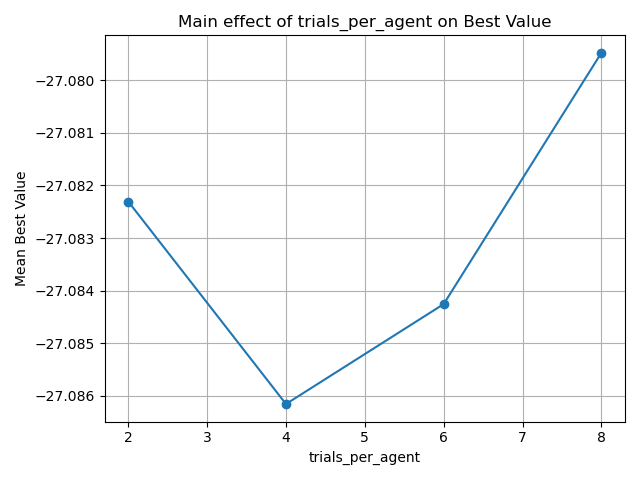
\includegraphics[scale=0.25]{potential10_trialsPerAgent}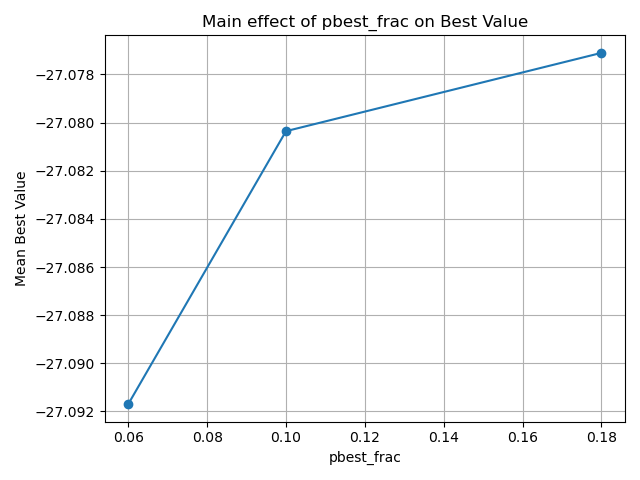
\includegraphics[scale=0.25]{potential10_pBestFrac}

\caption{Graphical representation of $\tau$, $\rho$, $\sigma,$ $t$ and
$\varphi$ for the “Lennard-Jones Potential, Dim:10” problem\protect\label{fig:graphicalLennard}}
\end{figure}
\begin{table}[H]
\caption{Sensitivity analysis of the method parameters for the ``Tersoff Potential
for model Si (C)'' problem\protect\label{tab:tersoffc}}

\centering{}%
\begin{tabular}{ccccccc}
\hline 
\textbf{Parameter} & \textbf{Value} & \textbf{Mean} & \textbf{Min} & \textbf{Max} & \textbf{Iters} & \textbf{Main effect range}\tabularnewline
\hline 
\hline 
\multirow{3}{*}{$\tau$} & 12 & -31.6851 & -34.1571 & -27.5111 & 3240 & \multirow{3}{*}{0.0171}\tabularnewline
\cline{2-6}
 & 18 & -31.6897 & -34.5056 & -27.9642 & 3240 & \tabularnewline
\cline{2-6}
 & 30 & -31.6725 & -34.1820 & -28.0777 & 3240 & \tabularnewline
\hline 
\multirow{3}{*}{$\rho$} & 0.05 & -31.6850 & -34.2058 & -27.6689 & 3240 & \multirow{3}{*}{0.0118}\tabularnewline
\cline{2-6}
 & 0.1 & -31.6752 & -34.5056 & -28.2521 & 3240 & \tabularnewline
\cline{2-6}
 & 0.2 & -31.6870 & -34.2775 & -27.5111 & 3240 & \tabularnewline
\hline 
\multirow{3}{*}{$\sigma$} & 0.1 & -31.6830 & -34.1571 & -27.5111 & 3240 & \multirow{3}{*}{0.0139}\tabularnewline
\cline{2-6}
 & 0.2 & -31.6890 & -34.5056 & -28.0084 & 3240 & \tabularnewline
\cline{2-6}
 & 0.3 & -31.6751 & -34.2775 & -27.6689 & 3240 & \tabularnewline
\hline 
\multirow{4}{*}{$t$} & 2 & -31.6994 & -34.2775 & -27.6689 & 3240 & \multirow{4}{*}{0.0524}\tabularnewline
\cline{2-6}
 & 4 & -31.7036 & -34.5056 & -28.0084 & 3240 & \tabularnewline
\cline{2-6}
 & 6 & -31.6753 & -34.1820 & -27.9642 & 3240 & \tabularnewline
\cline{2-6}
 & 8 & -31.6512 & -34.1365 & -27.5111 & 3240 & \tabularnewline
\hline 
\multirow{3}{*}{$\varphi$} & 0.06 & -31.6887 & -34.1365 & -27.5111 & 3240 & \multirow{3}{*}{0.0127}\tabularnewline
\cline{2-6}
 & 0.1 & -31.6825 & -34.1820 & -28.0777 & 3240 & \tabularnewline
\cline{2-6}
 & 0.18 & -31.6760 & -34.5056 & -27.6689 & 3240 & \tabularnewline
\hline 
\end{tabular}
\end{table}
\begin{figure}[H]
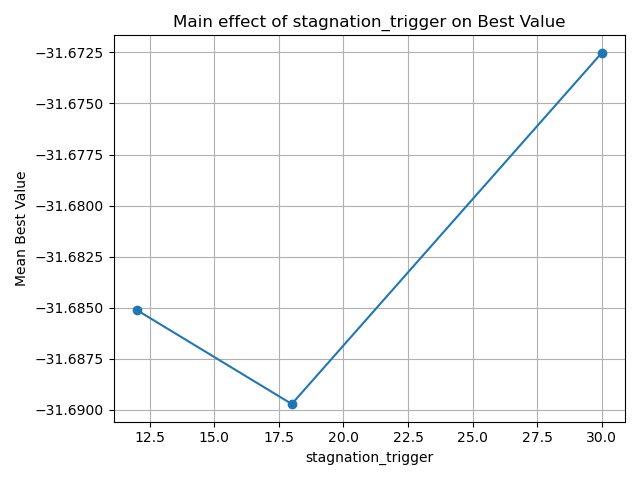
\includegraphics[scale=0.25]{tersoffc_stagnationTrigger}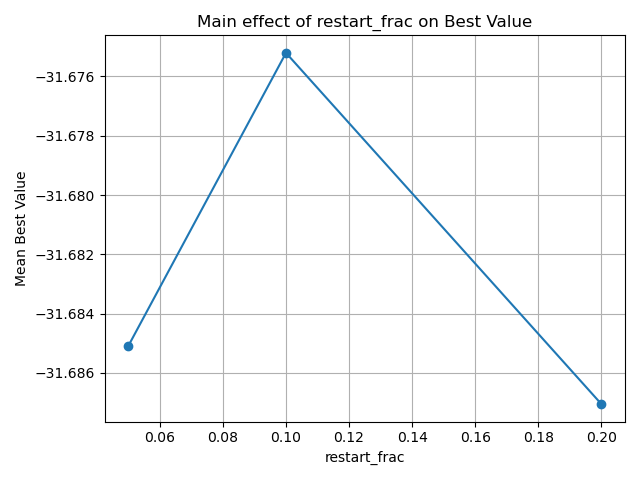
\includegraphics[scale=0.25]{tersoffc_resratFrac}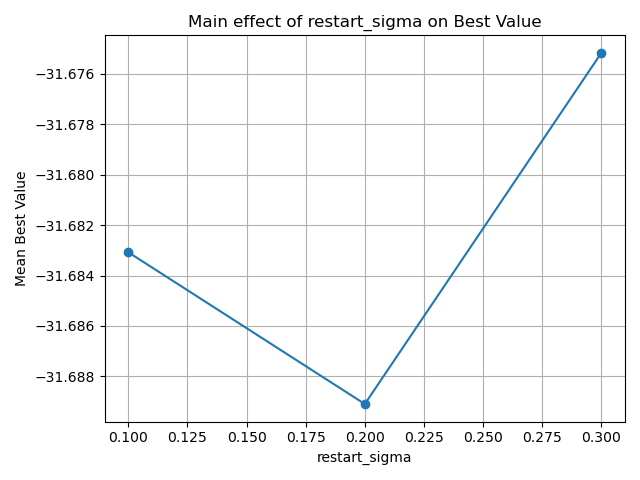
\includegraphics[scale=0.25]{tersoffc_restartSigma}

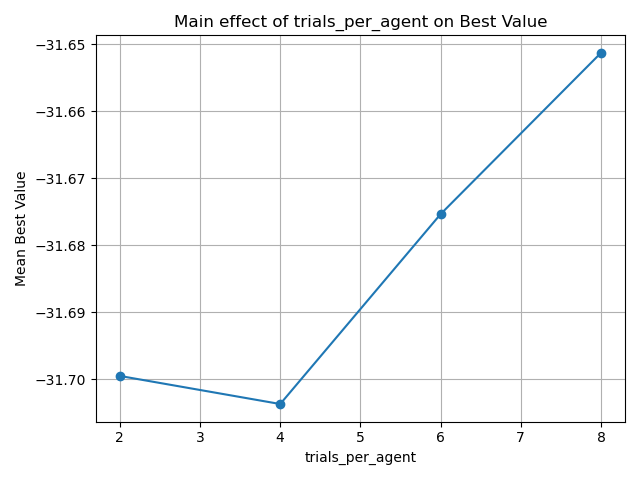
\includegraphics[scale=0.25]{tersoffc_trialPerAgent}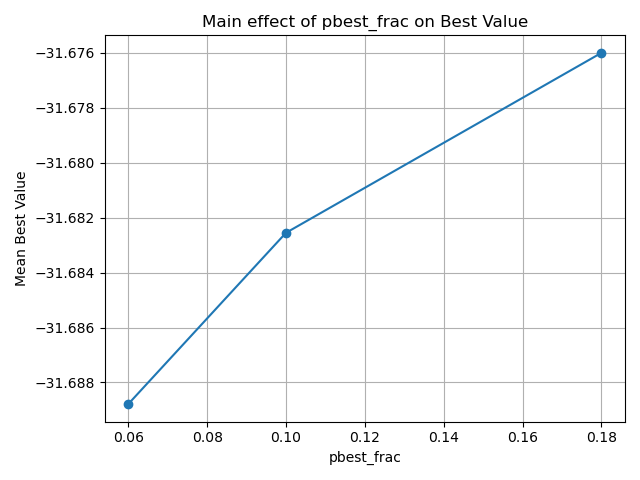
\includegraphics[scale=0.25]{tersoffc_pBestFrac}

\caption{Graphical representation of $\tau$, $\rho$, $\sigma,$ $t$ and
$\varphi$ for the “Tersoff Potential for model Si (C)” problem\protect\label{fig:graphicalTersoffc}}
\end{figure}
\begin{table}[H]
\caption{Sensitivity analysis of the method parameters for the ``Static Economic
Load Dispatch 1'' problem\protect\label{tab:eld}}

\centering{}%
\begin{tabular}{rrrrrrr|}
\hline 
\textbf{Parameter} & \textbf{Value} & \textbf{Mean} & \textbf{Min} & \textbf{Max} & \textbf{Iters} & \textbf{Main effect range}\tabularnewline
\hline 
\hline 
\multirow{3}{*}{{\footnotesize$\tau$}} & 12 & 2977.7669 & 2967.2491 & 3002.3335 & 3240 & \multirow{3}{*}{0.3580}\tabularnewline
\cline{2-6}
 & 18 & 2977.5983 & 2967.2491 & 3039.8430 & 3240 & \tabularnewline
\cline{2-6}
 & 30 & 2977.9563 & 2967.2491 & 3167.0430 & 3240 & \tabularnewline
\hline 
\multirow{3}{*}{{\footnotesize$\rho$}} & 0.05 & 2977.7981 & 2967.2491 & 3167.0430 & 3240 & \multirow{3}{*}{0.1440}\tabularnewline
\cline{2-6}
 & 0.1 & 2977.8338 & 2967.2491 & 3039.8430 & 3240 & \tabularnewline
\cline{2-6}
 & 0.2 & 2977.6897 & 2967.2491 & 3039.8430 & 3240 & \tabularnewline
\hline 
\multirow{3}{*}{{\footnotesize$\sigma$}} & 0.1 & 2977.7085 & 2967.2491 & 3167.0430 & 3240 & \multirow{3}{*}{0.1282}\tabularnewline
\cline{2-6}
 & 0.2 & 2977.8367 & 2967.2491 & 3031.7766 & 3240 & \tabularnewline
\cline{2-6}
 & 0.3 & 2977.7764 & 2967.2491 & 3039.8430 & 3240 & \tabularnewline
\hline 
\multirow{4}{*}{{\footnotesize$t$}} & 2 & 2977.6721 & 2967.2491 & 3039.8430 & 3240 & \multirow{4}{*}{0.1995}\tabularnewline
\cline{2-6}
 & 4 & 2977.7556 & 2967.2491 & 3039.8430 & 3240 & \tabularnewline
\cline{2-6}
 & 6 & 2977.7959 & 2967.2491 & 3039.8430 & 3240 & \tabularnewline
\cline{2-6}
 & 8 & 2977.8717 & 2967.2491 & 3167.0430 & 3240 & \tabularnewline
\hline 
\multirow{3}{*}{{\footnotesize$\varphi$}} & 0.06 & 2977.9287 & 2967.2491 & 3039.8430 & 3240 & \multirow{3}{*}{0.3351}\tabularnewline
\cline{2-6}
 & 0.1 & 2977.7994 & 2967.2491 & 3167.0430 & 3240 & \tabularnewline
\cline{2-6}
 & 0.18 & 2977.5935 & 2967.2491 & 3031.7766 & 3240 & \tabularnewline
\hline 
\end{tabular}
\end{table}
\begin{figure}[H]
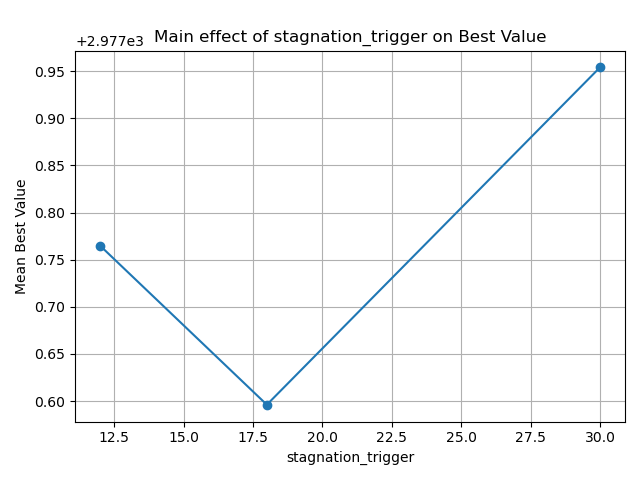
\includegraphics[scale=0.25]{eld_stagnationTrigger}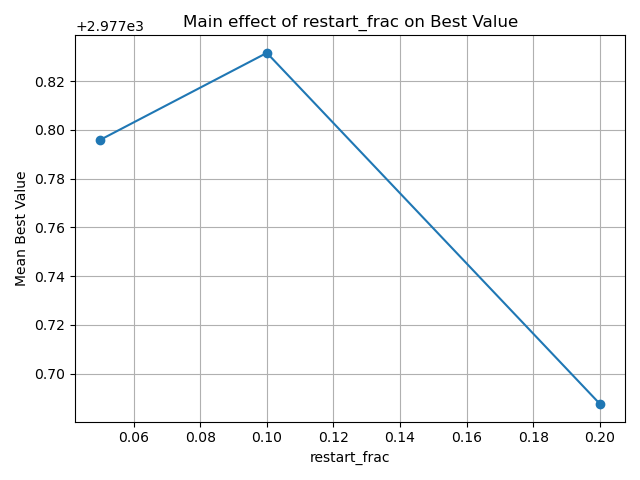
\includegraphics[scale=0.25]{eld_restartFrac}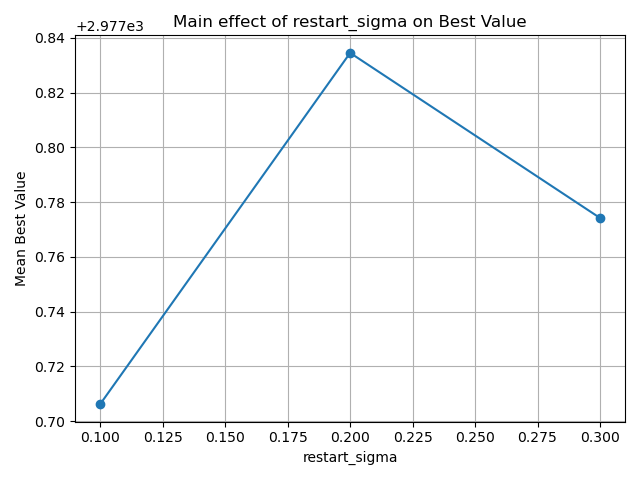
\includegraphics[scale=0.25]{eld_restartsigma}

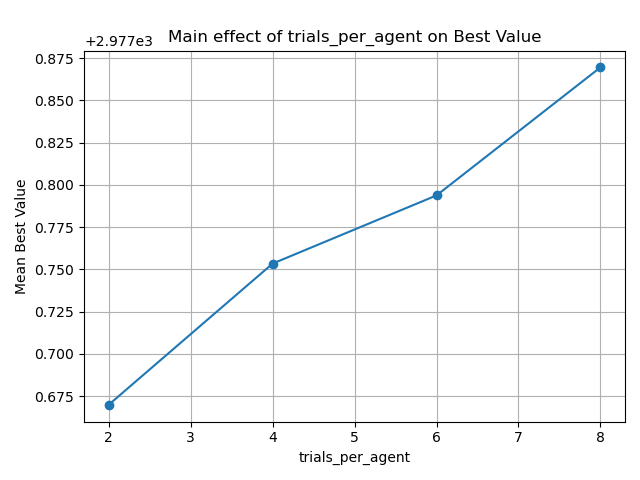
\includegraphics[scale=0.25]{eld_trialsPerAgent}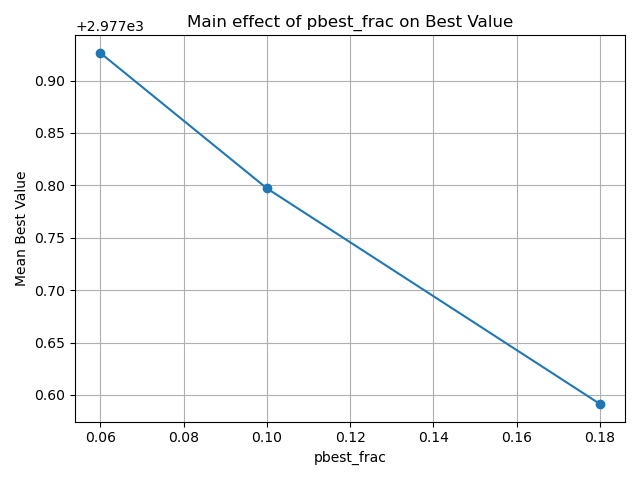
\includegraphics[scale=0.25]{eld_pBestFrac}

\caption{Graphical representation of $\tau$, $\rho$, $\sigma,$ $t$ and
$\varphi$ for the “Static Economic Load Dispatch 1” problem\protect\label{fig:graphicalEld}}
\end{figure}

The parameter sensitivity study probes the stability of TRIDENT-DE
under controlled variations of key hyperparameters and quantifies
whether reliability is preserved across heterogeneous operating conditions.
We focus on the stagnation counter before restart $\tau$, the restart
fraction $\rho$, the elite-centred Gaussian kick scale $\sigma$
at restart, the number of trials per agent $t$, and the top-p fraction
$\varphi$ that governs the pbest/1 sampling. Each factor is swept
over representative values around the defaults in Table \ref{tab:parameters}
while the remaining factors are kept fixed, and we record the impact
on mean performance, extrema, and the main-effect range for three
complementary test classes: a molecular Lennard-Jones cluster at $N$=10,
the Tersoff potential for silicon (model B), and the Static Economic
Load Dispatch (ELD-1) problem. This trio spans rugged, multimodal
physical landscapes and heavily constrained industrial testbeds, thereby
making observed trends transferable rather than instance-specific.
For Lennard-Jones, perturbations around $\tau$ =12/18/30, $\rho$
=0.05/0.1/0.2, $\sigma$ =0.1/0.2/0.3, $t$ =2/4/6/8, and $\varphi$
=0.06/0.10/0.18 induce only minor shifts in mean objective value and
very small main-effect ranges across all factors, indicating inherent
robustness of the method in this multimodal setting. The tight concentration
of means around \textasciitilde -27.08 together with the lack of
systematic movement in extremes suggests that the triple-operator
ensemble, the mild jDE-style control on $F$ and $C$, and the one-step
greedy line refinement act as dampers against parameter oversensitivity,
especially because the refinement reuses a precomputed direction at
negligible variance cost. These observations are evident in Table
\ref{tab:lennard} and Figure \ref{fig:graphicalLennard}. 

In the Tersoff-Si (model B) potential, the overall robustness pattern
persists, with the number of trials per agent $t$ showing the most
noticeable albeit still small effect on mean performance and main-effect
range. Increasing $t$ slightly improves exploitation of promising
directions, occasionally trading off diversity, yet exploration remains
safeguarded by adaptive micro-restarts, so the dynamics do not collapse.
The gentle drift in mean with $t$ does not overturn the defaults
of Table \ref{tab:parameters}, whereas $\rho$ and $\sigma$ exert
only marginal influence within the probed ranges, underscoring that
restarts serve as a safety valve rather than a dominant driver. The
quantitative evidence is given in Table \ref{tab:tersoffc} and Figure
\ref{fig:graphicalTersoffc}. 

The picture changes more distinctly for ELD-1. Here, the lack of time
coupling removes inter-temporal interactions, yet feasibility remains
tight due to the power-balance equality and unit output bounds. Depending
on the presence of valve-point effects, the landscape can be markedly
nonconvex, with ripple-like undulations around local extrema. In this
setting, the stagnation threshold $\tau$ still acts as a reliable
trigger for rejuvenation when the population gets trapped in shallow
basins, but its relative influence is smaller than in dynamic DED-type
problems because there are no time-linked plateaus reinforcing stagnation.
By contrast, the top-p fraction $\varphi$ becomes the primary control
knob: it governs how strongly the search is pulled toward p-best elites,
mediating the trade-off between aggressive exploitation near top units
and the preservation of diversity across alternative feasible corridors.
Increasing $t$ (trials per agent) further improves the use of local
directions without collapsing exploration, as adaptive micro-restarts
with calibrated $\rho$ and $\sigma$ inject gentle diversity whenever
stagnation is detected. The results in Table \ref{tab:eld} and the
corresponding figure \ref{fig:graphicalEld} indicate that defaults
around $\tau$ \ensuremath{\approx} 18 and $\varphi$ \ensuremath{\approx}
0.10 are safe operating points for ELD-1, small local retunings of
these two parameters can yield more stable quality jumps when valve-point
ripples make the landscape more “toothed,” without requiring adjustments
to $\rho$ and $\sigma$ beyond the probed ranges.

Taken together, the sensitivity profile shows that the defaults in
Table \ref{tab:parameters} are well-balanced across diverse problems:
$\rho$ and $\sigma$ regulate a gentle injection of diversity without
disrupting exploitation, $\varphi$ shapes the attraction lattice
of pbest/1 across multiple elites, and $t$ enhances the utility of
the already computed direction $z\rightarrow x\top$ at modest additional
cost. The small main-effect ranges observed in Lennard-Jones and Tersoff
confirm that the triple-operator design, combined with light jDE-style
jitter on $F$ and $C$, yields a self-stabilising regime in which
parameter effects are largely second-order. Conversely, in heavily
constrained energy scheduling, $\tau$ and $\varphi$ become active
control knobs, consistent with a landscape featuring broad plateaus
and tight feasibility margins. The practical implication is twofold:
first, the proposed defaults deliver portable reliability with minimal
pre-tuning, second, when constraints dominate, a narrow local retuning
of $\tau$ and $\varphi$ around their nominal values preserves the
best search rate without sacrificing stability. These conclusions
align with the architecture of TRIDENT-DE, where interactions among
three trial generators, one-step greedy refinement, and adaptive micro-restarts
distribute the burden of adaptation and, as a result, insulate the
system from sharp nonlinearities in any single hyperparameter.

\subsection{Analysis of Complexity of TRIDENT-DE\protect\label{subsec:Complexity}}

Below we provide a bullet-style specification of two real-world optimization
problems adopted as representative testbeds for the time-complexity
and scaling analysis of the proposed method, we summarise the key
decision variables, admissible bounds/domains, and objective functions,
and explicitly note relevant modeling assumptions and feasibility
penalty terms, so that the ensuing bullets serve as a quick “map”
of practical constraints and goals prior to the runtime evaluation.
\begin{itemize}
\item \textbf{GasCycle Thermal Cycle}

Vars: $\bm{x}=[T_{1},T_{3},P_{1},P_{3}]^{\top}$. \quad{}$r=P_{3}/P_{1},\ \gamma=1.4.$
\[
\eta(\bm{x})=1-r^{-(\gamma-1)/\gamma}\,\frac{T_{1}}{T_{3}},\qquad\min_{\bm{x}}f(\bm{x})=-\eta(\bm{x}).
\]
Bounds: $300\!\le\!T_{1}\!\le\!1500,\;1200\!\le\!T_{3}\!\le\!2000,\;1\!\le\!P_{1},P_{3}\!\le\!20.$

Penalty: infeasible $\Rightarrow f=10^{20}$.
\item \textbf{Tandem Space Trajectory} (MGA-1DSM, EVEEJ + 2$\times$Saturn)

Vars\textbf{ ($D{=}18$):} $\bm{x}=[t_{0},T_{1},T_{2},T_{3},T_{4},T_{5A},T_{5B},s_{1},s_{2},s_{3},s_{4},s_{5A},s_{5B},r_{p},k_{A1},k_{A2},k_{B1},k_{B2}]^{\top}$.
\[
\begin{aligned} & 7000\le t_{0}\le10000,\\
 & 30\le T_{1}\le500,\;30\le T_{2}\le600,\;30\le T_{3}\le1200,\\
 & 30\le T_{4}\le1600,\;30\le T_{5A},T_{5B}\le2000,\\
 & 0\le s_{1..4},s_{5A},s_{5B},r_{p},k_{A1},k_{A2},k_{B1},k_{B2}\le1.
\end{aligned}
\]
Objective: 
\[
\min_{\bm{x}}\ \Delta V_{\text{tot}}=\Delta V_{\text{launch}}(T_{1})+\Delta V_{\text{legs}}(T_{1}{:}T_{4})+\Delta V_{A}+\Delta V_{B}+\Delta V_{\text{DSM}}(\bm{s},r_{p})-G_{\text{GA}}-G_{J}+P_{\text{hard}}+P_{\text{soft}},
\]
\medskip{}
 
\[
P_{\text{soft}}=\beta\max\!\Big\{0,\ (T_{1}{+}\cdots{+}T_{4}+\tfrac{1}{2}(T_{5A}{+}T_{5B}))-3500\Big\}.
\]
Notes: $\Delta V_{\text{launch}}$ decreases (log-like) in $T_{1}$
($\ge6$ km/s floor), leg/branch costs decrease with TOF.

\medskip{}

\end{itemize}
The time-complexity Figure \ref{fig:complexity} reveals an almost
linear growth of wall-clock time with respect to problem size (40-400)
for both GasCycle Thermal Cycle and Tandem Space Trajectory. The monotonic
trend and near-constant increments per size step indicate that the
proposed architecture scales effectively with $O(n)$ in the investigated
size parameter, with no signs of exponential or strongly super-linear
behavior. Across the two cases, Tandem Space Trajectory consistently
exhibits slightly higher times, which is naturally explained by a
larger per-evaluation cost of the underlying simulator/objective in
that domain. In other words, the dominant contributor to total runtime
is the evaluation cost, while the search mechanism itself preserves
an approximately constant slope with respect to size. The absence
of kinks or abrupt escalations at larger sizes further suggests that
components such as the triple trial-vector ensemble, the one-step
greedy line refinement, and the adaptive micro-restarts do not introduce
hidden overhead that would manifest as degraded asymptotic scaling.
Practically, the method remains predictable and efficient as the problem
grows, with performance primarily governed by the problem-dependent
evaluation burden. The mild, roughly constant offset between the two
benchmarks over the 40-400 range reinforces the view that this is
a domain-dependent additive cost rather than a change in the algorithm’s
scaling rate. Overall, the evidence supports a favorable scaling profile:
linear complexity in the examined size parameter, stability under
heavier loads, and a clean separation between a stable algorithmic
overhead and the variable evaluation cost imposed by each application.

\begin{figure}[H]
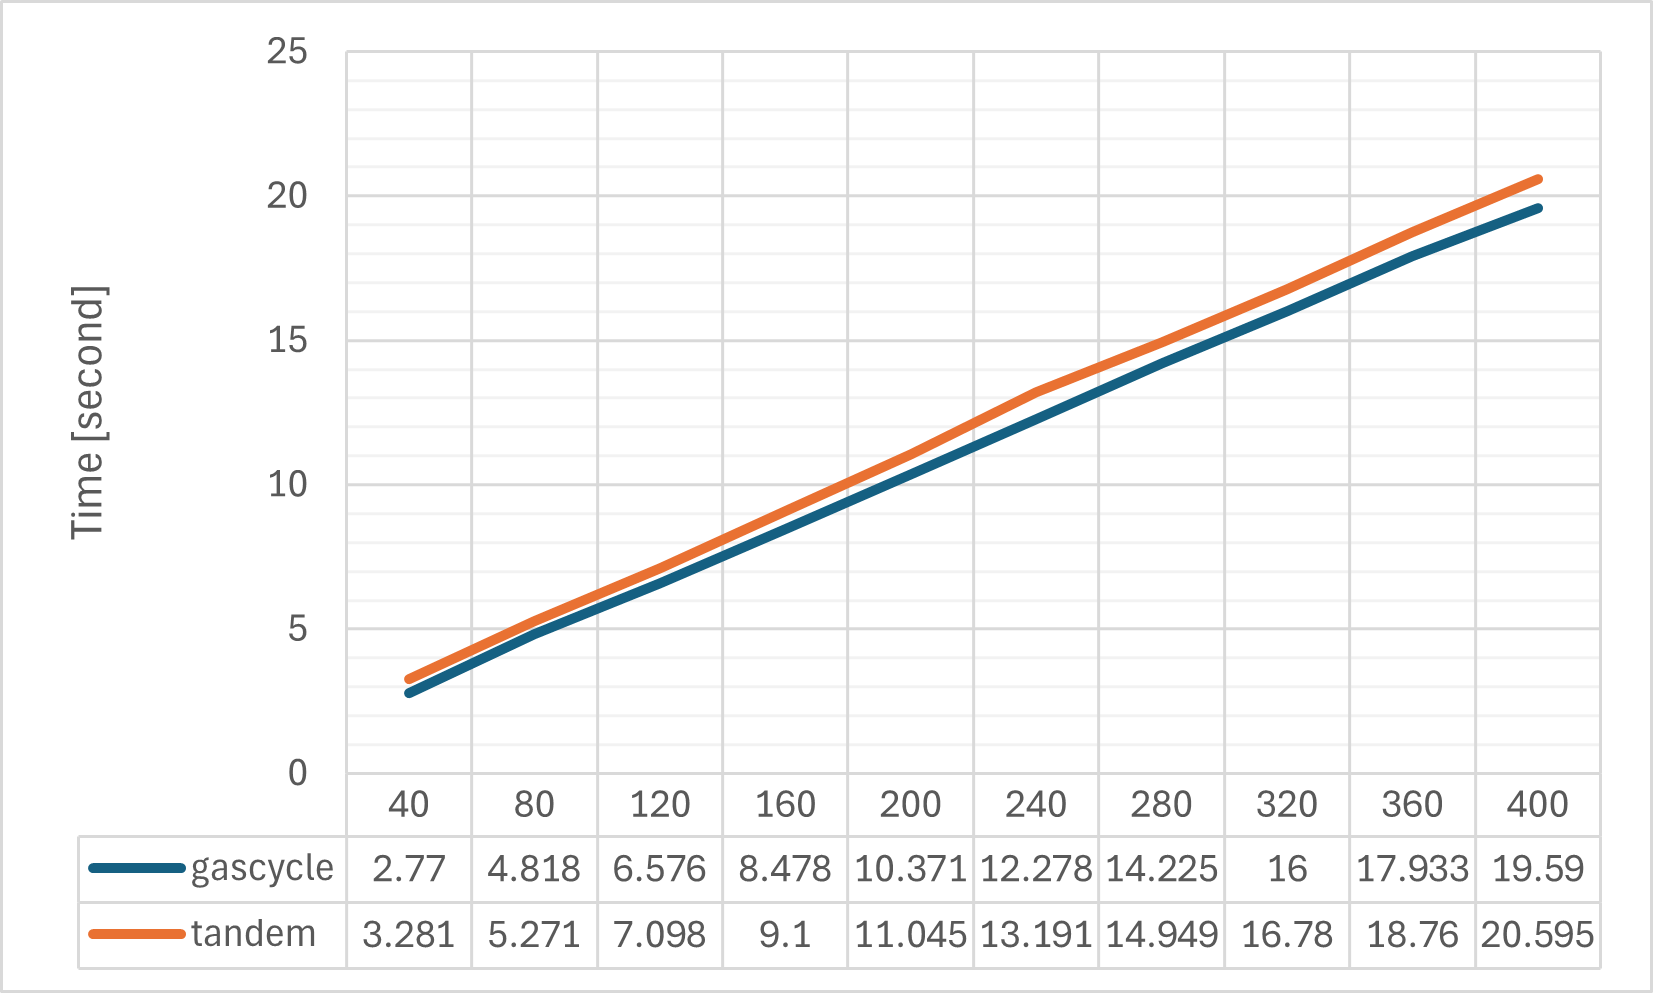
\includegraphics{complexity}\caption{Time scaling under a fixed iteration budget\protect\label{fig:complexity}}

\end{figure}


\subsection{Comparative performance analysis of TRIDENT-DE \protect\label{subsec:Experiments}}

This section introduces the experimental component that assesses the
proposed method across alternative configurations and problem sets,
emphasizing behavioral consistency and reproducibility. Table \ref{tab:methodsComparison}
compiles the corresponding comparative figures and summary evaluation
metrics.

\begin{table}[H]
\caption{Comparison Based on Best and Mean after 1.5e+5 FEs\protect\label{tab:methodsComparison}}

\begin{tabular}{ccccccccc}
\hline 
 & \begin{cellvarwidth}[t]
\centering
{\tiny\textbf{TRIDENT-DE}}{\tiny\par}

{\tiny\textbf{Best/Mean}}
\end{cellvarwidth} & \begin{cellvarwidth}[t]
\centering
{\tiny\textbf{UDE3}}{\tiny\par}

{\tiny\textbf{Best/Mean}}
\end{cellvarwidth} & \begin{cellvarwidth}[t]
\centering
{\tiny\textbf{EA4Eig}}{\tiny\par}

{\tiny\textbf{Best/Mean}}
\end{cellvarwidth} & \begin{cellvarwidth}[t]
\centering
{\tiny\textbf{mLSHADE\_RL}}{\tiny\par}

{\tiny\textbf{Best/Mean}}
\end{cellvarwidth} & \begin{cellvarwidth}[t]
\centering
{\tiny\textbf{SaDE}}{\tiny\par}

{\tiny\textbf{Best/Mean}}
\end{cellvarwidth} & \begin{cellvarwidth}[t]
\centering
{\tiny\textbf{CMA-ES}}{\tiny\par}

{\tiny\textbf{Best/Mean}}
\end{cellvarwidth} & \begin{cellvarwidth}[t]
\centering
{\tiny\textbf{jDE}}{\tiny\par}

{\tiny\textbf{Best/Mean}}
\end{cellvarwidth} & \begin{cellvarwidth}[t]
\centering
{\tiny\textbf{CLPSO}}{\tiny\par}

{\tiny\textbf{Best/Mean}}
\end{cellvarwidth}\tabularnewline
\hline 
\hline 
\multirow{2}{*}{\begin{cellvarwidth}[t]
\centering
{\tiny\textbf{Lennard-Jones}}{\tiny\par}

{\tiny\textbf{Potential (10 atoms)}}
\end{cellvarwidth}} & {\tiny -28.42253189} & {\tiny -17.60964115} & {\tiny -22.47842596} & {\tiny -28.42252711} & {\tiny -22.86077544} & {\tiny -28.42253189} & {\tiny -15.91366007} & {\tiny -16.59269921}\tabularnewline
\cline{2-9}
 & {\tiny -27.19833972} & {\tiny -16.33758634} & {\tiny -19.48663385} & {\tiny -23.77189104} & {\tiny -21.22806787} & {\tiny -27.52754934} & {\tiny -13.75563015} & {\tiny -13.55503647}\tabularnewline
\hline 
\multirow{2}{*}{\begin{cellvarwidth}[t]
\centering
{\tiny\textbf{Lennard-Jones}}{\tiny\par}

{\tiny\textbf{Potential (13 atoms)}}
\end{cellvarwidth}} & {\tiny -41.39220729} & {\tiny -21.90945922} & {\tiny -28.01101572} & {\tiny -40.6992486} & {\tiny -29.31393114} & {\tiny -44.32680142} & {\tiny -18.77073675} & {\tiny -18.00250514}\tabularnewline
\cline{2-9}
 & {\tiny -39.14390841} & {\tiny -19.49372047} & {\tiny -24.58810405} & {\tiny -30.67706246} & {\tiny -27.48874237} & {\tiny -41.44245617} & {\tiny -15.4243072} & {\tiny -15.86691988}\tabularnewline
\hline 
\multirow{2}{*}{\begin{cellvarwidth}[t]
\centering
{\tiny\textbf{Lennard-Jones}}{\tiny\par}

{\tiny\textbf{Potential (38 atoms)}}
\end{cellvarwidth}} & {\tiny -125.1886792} & {\tiny -2.015038465} & {\tiny -55.05415428} & {\tiny -120.0680452} & {\tiny -68.91313107} & {\tiny -167.7369019} & {\tiny 9186.25096} & {\tiny 330.9934848}\tabularnewline
\cline{2-9}
 & {\tiny -107.1751456} & {\tiny 140.2211284} & {\tiny -3.350181902} & {\tiny -73.95117658} & {\tiny -45.80265994} & {\tiny -163.6091673} & {\tiny 9186.25096} & {\tiny 1087.035295}\tabularnewline
\hline 
\multirow{2}{*}{\begin{cellvarwidth}[t]
\centering
{\tiny\textbf{Tersoff Potential}}{\tiny\par}

{\tiny\textbf{for model Si (B)}}
\end{cellvarwidth}} & {\tiny -28.93480467} & {\tiny -25.43447342} & {\tiny -26.90746941} & {\tiny -28.12281867} & {\tiny -26.65687822} & {\tiny -28.33045002} & {\tiny -24.75133772} & {\tiny -22.67387001}\tabularnewline
\cline{2-9}
 & {\tiny -27.70615763} & {\tiny -23.30318979} & {\tiny -24.69059932} & {\tiny -25.49977206} & {\tiny -25.27422603} & {\tiny -27.38991233} & {\tiny -22.94168766} & {\tiny -21.21150428}\tabularnewline
\hline 
\multirow{2}{*}{\begin{cellvarwidth}[t]
\centering
{\tiny\textbf{Tersoff Potential}}{\tiny\par}

{\tiny\textbf{for model Si (C)}}
\end{cellvarwidth}} & {\tiny -33.8820283} & {\tiny -29.30227462} & {\tiny -30.88865174} & {\tiny -31.70444684} & {\tiny -30.94469385} & {\tiny -32.50963421} & {\tiny -29.44789882} & {\tiny -26.88039528}\tabularnewline
\cline{2-9}
 & {\tiny -31.91749393} & {\tiny -27.53891341} & {\tiny -29.0199918} & {\tiny -29.44303263} & {\tiny -29.70029831} & {\tiny -31.53772845} & {\tiny -29.44789882} & {\tiny -24.653633}\tabularnewline
\hline 
\multirow{2}{*}{\begin{cellvarwidth}[t]
\centering
{\tiny\textbf{Parameter Estimation for}}{\tiny\par}

{\tiny\textbf{Frequency-Modulated Sound Waves}}
\end{cellvarwidth}} & {\tiny 0.116157535} & {\tiny 0} & {\tiny 0.15272453} & {\tiny 0.116157535} & {\tiny 0.148007602} & {\tiny 0.210122687} & {\tiny 0} & {\tiny 0.131483748}\tabularnewline
\cline{2-9}
 & {\tiny 0.134324544} & {\tiny 0.103406319} & {\tiny 0.213099692} & {\tiny 0.208210846} & {\tiny 0.148007602} & {\tiny 0.267329914} & {\tiny 0.132539923} & {\tiny 0.212498169}\tabularnewline
\hline 
\multirow{2}{*}{\begin{cellvarwidth}[t]
\centering
{\tiny\textbf{Circular Antenna}}{\tiny\par}

{\tiny\textbf{Array Design}}
\end{cellvarwidth}} & {\tiny 0.006809638} & {\tiny 0.006809665} & {\tiny 0.006809638} & {\tiny 0.006809662} & {\tiny 0.006814682} & {\tiny 0.007253731} & {\tiny 0.00681715} & {\tiny 0.006933401}\tabularnewline
\cline{2-9}
 & {\tiny 0.006809683} & {\tiny 0.006817385} & {\tiny 0.006809638} & {\tiny 0.006825338} & {\tiny 0.00790701} & {\tiny 0.008755359} & {\tiny 0.006835764} & {\tiny 0.051815518}\tabularnewline
\hline 
\multirow{2}{*}{\begin{cellvarwidth}[t]
\centering
{\tiny\textbf{Spread Spectrum Radar}}{\tiny\par}

{\tiny\textbf{Polyphase Code Design}}
\end{cellvarwidth}} & {\tiny 0.014426836} & {\tiny 0.953872709} & {\tiny 0.601567824} & {\tiny 0.074552911} & {\tiny 0.550837019} & {\tiny 0.062519409} & {\tiny 1.005739785} & {\tiny 0.860294378}\tabularnewline
\cline{2-9}
 & {\tiny 0.26254527} & {\tiny 1.206577385} & {\tiny 0.869257599} & {\tiny 0.535028919} & {\tiny 0.803527605} & {\tiny 0.197713522} & {\tiny 1.331416957} & {\tiny 1.273200439}\tabularnewline
\hline 
\multirow{2}{*}{\begin{cellvarwidth}[t]
\centering
{\tiny\textbf{Cassini 2: Spacecraft Trajectory}}{\tiny\par}

{\tiny\textbf{Optimization Problem}}
\end{cellvarwidth}} & {\tiny 0} & {\tiny 0.000926598} & {\tiny 0} & {\tiny 0} & {\tiny 0.039231105} & {\tiny 0} & {\tiny 0.000026961} & {\tiny 1.22633022}\tabularnewline
\cline{2-9}
 & {\tiny 0.000011205} & {\tiny 0.008206106} & {\tiny 0} & {\tiny 0.00001729} & {\tiny 0.070230417} & {\tiny 5.929143722} & {\tiny 0.000285411} & {\tiny 3.639687905}\tabularnewline
\hline 
\multirow{2}{*}{\begin{cellvarwidth}[t]
\centering
{\tiny\textbf{Wireless Coverage}}{\tiny\par}

{\tiny\textbf{Antenna Placement}}
\end{cellvarwidth}} & {\tiny 0.946350736} & {\tiny 0.946350736} & {\tiny 0.946655032} & {\tiny 0.946350736} & {\tiny 0.946361987} & {\tiny 1.18939375} & {\tiny 0.946350736} & {\tiny 0.946365969}\tabularnewline
\cline{2-9}
 & {\tiny 0.94662124} & {\tiny 0.946502884} & {\tiny 0.946659575} & {\tiny 0.946875107} & {\tiny 0.946688757} & {\tiny 1.190699803} & {\tiny 0.946401452} & {\tiny 0.946727502}\tabularnewline
\hline 
\multirow{2}{*}{\begin{cellvarwidth}[t]
\centering
{\tiny\textbf{Transmission Network}}{\tiny\par}

{\tiny\textbf{Expansion Planning}}
\end{cellvarwidth}} & {\tiny 4.485304003} & {\tiny 4.485295106} & {\tiny 4.485292926} & {\tiny 4.485292926} & {\tiny 4.485299525} & {\tiny 4.485292926} & {\tiny 4.485292926} & {\tiny 4.486699087}\tabularnewline
\cline{2-9}
 & {\tiny 4.485292926} & {\tiny 4.485304003} & {\tiny 4.485292926} & {\tiny 4.485292926} & {\tiny 4.485311924} & {\tiny 4.485292948} & {\tiny 4.485292926} & {\tiny 4.495857336}\tabularnewline
\hline 
\multirow{2}{*}{\begin{cellvarwidth}[t]
\centering
{\tiny\textbf{Dynamic}}{\tiny\par}

{\tiny\textbf{Economic Dispatch 1}}
\end{cellvarwidth}} & {\tiny 130850.0389} & {\tiny 130693.5423} & {\tiny 130694.29} & {\tiny 130882.0646} & {\tiny 131010.8769} & {\tiny 130650.9354} & {\tiny 131225.2453} & {\tiny 131834.4235}\tabularnewline
\cline{2-9}
 & {\tiny 130931.1074} & {\tiny 130717.6052} & {\tiny 130862.9893} & {\tiny 130955.331} & {\tiny 131099.1959} & {\tiny 130654.2758} & {\tiny 131225.2453} & {\tiny 132151.5397}\tabularnewline
\hline 
\multirow{2}{*}{\begin{cellvarwidth}[t]
\centering
{\tiny\textbf{Dynamic}}{\tiny\par}

{\tiny\textbf{Economic Dispatch 2}}
\end{cellvarwidth}} & {\tiny 165980.9574} & {\tiny 164946.164} & {\tiny 172067.4426} & {\tiny 167519.3281} & {\tiny 167908.0605} & {\tiny 165847.1092} & {\tiny 186121.2812} & {\tiny 177120.3822}\tabularnewline
\cline{2-9}
 & {\tiny 166478.1534} & {\tiny 165614.9256} & {\tiny 172931.6964} & {\tiny 168275.5429} & {\tiny 168495.9731} & {\tiny 166233.691} & {\tiny 190793.5621} & {\tiny 178190.4198}\tabularnewline
\hline 
\multirow{2}{*}{\begin{cellvarwidth}[t]
\centering
{\tiny\textbf{Static Economic}}{\tiny\par}

{\tiny\textbf{Load Dispatch 1}}
\end{cellvarwidth}} & {\tiny 2967.249196} & {\tiny 2967.249196} & {\tiny 2979.803369} & {\tiny 2967.249196} & {\tiny 2967.249196} & {\tiny 2967.249586} & {\tiny 2967.249196} & {\tiny 2967.249197}\tabularnewline
\cline{2-9}
 & {\tiny 2975.721343} & {\tiny 2976.057657} & {\tiny 2979.803369} & {\tiny 2976.956221} & {\tiny 2976.139816} & {\tiny 3108.931917} & {\tiny 2967.659992} & {\tiny 2973.33009}\tabularnewline
\hline 
\multirow{2}{*}{\begin{cellvarwidth}[t]
\centering
{\tiny\textbf{Static Economic}}{\tiny\par}

{\tiny\textbf{Load Dispatch 2}}
\end{cellvarwidth}} & {\tiny 17879.73679} & {\tiny 17864.69687} & {\tiny 18006.65976} & {\tiny 17882.28384} & {\tiny 17892.38129} & {\tiny 17960.84734} & {\tiny 17867.57447} & {\tiny 17910.47794}\tabularnewline
\cline{2-9}
 & {\tiny 17928.65603} & {\tiny 17890.83413} & {\tiny 18063.12085} & {\tiny 17950.15892} & {\tiny 17958.94204} & {\tiny 18077.58006} & {\tiny 17992.09486} & {\tiny 18089.83526}\tabularnewline
\hline 
\multirow{2}{*}{\begin{cellvarwidth}[t]
\centering
{\tiny\textbf{Static Economic}}{\tiny\par}

{\tiny\textbf{Load Dispatch 3}}
\end{cellvarwidth}} & {\tiny 32367.57735} & {\tiny 32367.57735} & {\tiny 32415.80367} & {\tiny 32367.57765} & {\tiny 32376.02197} & {\tiny 32645.34102} & {\tiny 32391.64981} & {\tiny 32384.85409}\tabularnewline
\cline{2-9}
 & {\tiny 32440.87752} & {\tiny 32400.86337} & {\tiny 32573.03572} & {\tiny 32491.57235} & {\tiny 32491.28971} & {\tiny 32867.1729} & {\tiny 32476.58405} & {\tiny 32532.19143}\tabularnewline
\hline 
\multirow{2}{*}{\begin{cellvarwidth}[t]
\centering
{\tiny\textbf{Static Economic}}{\tiny\par}

{\tiny\textbf{Load Dispatch 4}}
\end{cellvarwidth}} & {\tiny 121071.4654} & {\tiny 121066.9247} & {\tiny 121197.2468} & {\tiny 121085.9922} & {\tiny 121195.4656} & {\tiny 122350.1013} & {\tiny 121234.0466} & {\tiny 121328.7006}\tabularnewline
\cline{2-9}
 & {\tiny 121422.9908} & {\tiny 121197.2468} & {\tiny 121545.1315} & {\tiny 121308.5801} & {\tiny 121517.4918} & {\tiny 122957.6217} & {\tiny 121526.7414} & {\tiny 121541.4182}\tabularnewline
\hline 
\multirow{2}{*}{\begin{cellvarwidth}[t]
\centering
{\tiny\textbf{Static Economic}}{\tiny\par}

{\tiny\textbf{Load Dispatch 5}}
\end{cellvarwidth}} & {\tiny 508663.8176} & {\tiny 508661.3113} & {\tiny 508872.6908} & {\tiny 508851.668} & {\tiny 508985.9092} & {\tiny 508717.1467} & {\tiny 511174.5326} & {\tiny 509025.7426}\tabularnewline
\cline{2-9}
 & {\tiny 508703.0424} & {\tiny 508676.4938} & {\tiny 508986.6092} & {\tiny 508988.5396} & {\tiny 509125.2079} & {\tiny 508770.1661} & {\tiny 562012.6548} & {\tiny 509080.3439}\tabularnewline
\hline 
\end{tabular}
\end{table}
\begin{table}[H]
\caption{Detailed Ranking of Algorithms Based on Best after 1.5e+5 FEs\protect\label{tab:rank_best}}
 {\scriptsize{}%
\begin{tabular}{ccccccccc}
\toprule 
 & {\scriptsize\textbf{TRIDENT-DE}} & {\scriptsize\textbf{UDE3}} & {\scriptsize\textbf{EA4Eig}} & {\scriptsize\textbf{mLSHADE\_RL}} & {\scriptsize\textbf{SaDE}} & {\scriptsize\textbf{CMA-ES}} & {\scriptsize\textbf{jDE}} & {\scriptsize\textbf{CLPSO}}\tabularnewline
\midrule 
\begin{cellvarwidth}[t]
\centering
{\tiny\textbf{Lennard-Jones}}{\tiny\par}

{\tiny\textbf{Potential (10 atoms)}}
\end{cellvarwidth} & {\tiny\textcolor{green}{1}}{\tiny{} } & {\tiny 6 } & {\tiny 5 } & {\tiny 3 } & {\tiny 4 } & {\tiny\textcolor{green}{1}}{\tiny{} } & {\tiny 8 } & {\tiny 7 }\tabularnewline
\midrule 
\begin{cellvarwidth}[t]
\centering
{\tiny\textbf{Lennard-Jones}}{\tiny\par}

{\tiny\textbf{Potential (13 atoms)}}
\end{cellvarwidth} & {\tiny\textcolor{blue}{2}}{\tiny{} } & {\tiny 6 } & {\tiny 5 } & {\tiny 3 } & {\tiny 4 } & {\tiny\textcolor{green}{1}}{\tiny{} } & {\tiny 7 } & {\tiny 8 }\tabularnewline
\midrule 
\begin{cellvarwidth}[t]
\centering
{\tiny\textbf{Lennard-Jones}}{\tiny\par}

{\tiny\textbf{Potential (38 atoms)}}
\end{cellvarwidth} & {\tiny\textcolor{blue}{2}}{\tiny{} } & {\tiny 6 } & {\tiny 5 } & {\tiny 3 } & {\tiny 4 } & {\tiny\textcolor{green}{1}}{\tiny{} } & {\tiny 8 } & {\tiny 7 }\tabularnewline
\midrule 
\begin{cellvarwidth}[t]
\centering
{\tiny\textbf{Tersoff Potential}}{\tiny\par}

{\tiny\textbf{for model Si (B)}}
\end{cellvarwidth} & {\tiny\textcolor{green}{1}}{\tiny{} } & {\tiny 6 } & {\tiny 4 } & {\tiny 3 } & {\tiny 5 } & {\tiny\textcolor{blue}{2}}{\tiny{} } & {\tiny 7 } & {\tiny 8 }\tabularnewline
\midrule 
\begin{cellvarwidth}[t]
\centering
{\tiny\textbf{Tersoff Potential}}{\tiny\par}

{\tiny\textbf{for model Si (C)}}
\end{cellvarwidth} & {\tiny\textcolor{green}{1}}{\tiny{} } & {\tiny 7 } & {\tiny 5 } & {\tiny 3 } & {\tiny 4 } & {\tiny\textcolor{blue}{2}}{\tiny{} } & {\tiny 6 } & {\tiny 8 }\tabularnewline
\midrule 
\begin{cellvarwidth}[t]
\centering
{\tiny\textbf{Parameter Estimation for}}{\tiny\par}

{\tiny\textbf{Frequency-Modulated Sound Waves}}
\end{cellvarwidth} & {\tiny 3 } & {\tiny\textcolor{green}{1}}{\tiny{} } & {\tiny 7 } & {\tiny 3 } & {\tiny 6 } & {\tiny 8 } & {\tiny\textcolor{green}{1}}{\tiny{} } & {\tiny 5 }\tabularnewline
\midrule 
\begin{cellvarwidth}[t]
\centering
{\tiny\textbf{Circular Antenna}}{\tiny\par}

{\tiny\textbf{Array Design}}
\end{cellvarwidth} & {\tiny\textcolor{green}{1}}{\tiny{} } & {\tiny 4 } & {\tiny\textcolor{blue}{2}}{\tiny{} } & {\tiny 3 } & {\tiny 5 } & {\tiny 8 } & {\tiny 6 } & {\tiny 7 }\tabularnewline
\midrule 
\begin{cellvarwidth}[t]
\centering
{\tiny\textbf{Spread Spectrum Radar}}{\tiny\par}

{\tiny\textbf{Polyphase Code Design}}
\end{cellvarwidth} & {\tiny\textcolor{green}{1}}{\tiny{} } & {\tiny 7 } & {\tiny 5 } & {\tiny 3 } & {\tiny 4 } & {\tiny\textcolor{blue}{2}}{\tiny{} } & {\tiny 8 } & {\tiny 6 }\tabularnewline
\midrule 
\begin{cellvarwidth}[t]
\centering
{\tiny\textbf{Cassini 2: Spacecraft Trajectory}}{\tiny\par}

{\tiny\textbf{Optimization Problem}}
\end{cellvarwidth} & {\tiny\textcolor{green}{1}}{\tiny{} } & {\tiny 6 } & {\tiny\textcolor{green}{1}}{\tiny{} } & {\tiny\textcolor{green}{1}}{\tiny{} } & {\tiny 7 } & {\tiny\textcolor{green}{1}}{\tiny{} } & {\tiny 5 } & {\tiny 8 }\tabularnewline
\midrule 
\begin{cellvarwidth}[t]
\centering
{\tiny\textbf{Wireless Coverage}}{\tiny\par}

{\tiny\textbf{Antenna Placement}}
\end{cellvarwidth} & {\tiny\textcolor{green}{1}}{\tiny{} } & {\tiny\textcolor{green}{1}}{\tiny{} } & {\tiny 7 } & {\tiny\textcolor{green}{1}}{\tiny{} } & {\tiny 5 } & {\tiny 8 } & {\tiny\textcolor{green}{1}}{\tiny{} } & {\tiny 6 }\tabularnewline
\midrule 
\begin{cellvarwidth}[t]
\centering
{\tiny\textbf{Transmission Network}}{\tiny\par}

{\tiny\textbf{Expansion Planning}}
\end{cellvarwidth} & {\tiny 7 } & {\tiny 5 } & {\tiny\textcolor{green}{1}}{\tiny{} } & {\tiny\textcolor{green}{1}}{\tiny{} } & {\tiny 6 } & {\tiny\textcolor{green}{1}}{\tiny{} } & {\tiny\textcolor{green}{1}}{\tiny{} } & {\tiny 8 }\tabularnewline
\midrule 
\begin{cellvarwidth}[t]
\centering
{\tiny\textbf{Dynamic}}{\tiny\par}

{\tiny\textbf{Economic Dispatch 1}}
\end{cellvarwidth} & {\tiny 4 } & {\tiny\textcolor{blue}{2}}{\tiny{} } & {\tiny 3 } & {\tiny 5 } & {\tiny 6 } & {\tiny\textcolor{green}{1}}{\tiny{} } & {\tiny 7 } & {\tiny 8 }\tabularnewline
\midrule 
\begin{cellvarwidth}[t]
\centering
{\tiny\textbf{Dynamic}}{\tiny\par}

{\tiny\textbf{Economic Dispatch 2}}
\end{cellvarwidth} & {\tiny 3 } & {\tiny\textcolor{green}{1}}{\tiny{} } & {\tiny 6 } & {\tiny 4 } & {\tiny 5 } & {\tiny\textcolor{blue}{2}}{\tiny{} } & {\tiny 8 } & {\tiny 7 }\tabularnewline
\midrule 
\begin{cellvarwidth}[t]
\centering
{\tiny\textbf{Static Economic}}{\tiny\par}

{\tiny\textbf{Load Dispatch 1}}
\end{cellvarwidth} & {\tiny\textcolor{green}{1}}{\tiny{} } & {\tiny\textcolor{green}{1}}{\tiny{} } & {\tiny 8 } & {\tiny\textcolor{green}{1}}{\tiny{} } & {\tiny\textcolor{green}{1}}{\tiny{} } & {\tiny 7 } & {\tiny\textcolor{green}{1}}{\tiny{} } & {\tiny 6 }\tabularnewline
\midrule 
\begin{cellvarwidth}[t]
\centering
{\tiny\textbf{Static Economic}}{\tiny\par}

{\tiny\textbf{Load Dispatch 2}}
\end{cellvarwidth} & {\tiny 3 } & {\tiny\textcolor{green}{1}}{\tiny{} } & {\tiny 8 } & {\tiny 4 } & {\tiny 5 } & {\tiny 7 } & {\tiny\textcolor{blue}{2}}{\tiny{} } & {\tiny 6 }\tabularnewline
\midrule 
\begin{cellvarwidth}[t]
\centering
{\tiny\textbf{Static Economic}}{\tiny\par}

{\tiny\textbf{Load Dispatch 3}}
\end{cellvarwidth} & {\tiny\textcolor{green}{1}}{\tiny{} } & {\tiny\textcolor{green}{1}}{\tiny{} } & {\tiny 7 } & {\tiny 3 } & {\tiny 4 } & {\tiny 8 } & {\tiny 6 } & {\tiny 5 }\tabularnewline
\midrule 
\begin{cellvarwidth}[t]
\centering
{\tiny\textbf{Static Economic}}{\tiny\par}

{\tiny\textbf{Load Dispatch 4}}
\end{cellvarwidth} & {\tiny\textcolor{blue}{2}}{\tiny{} } & {\tiny\textcolor{green}{1}}{\tiny{} } & {\tiny 5 } & {\tiny 3 } & {\tiny 4 } & {\tiny 8 } & {\tiny 6 } & {\tiny 7 }\tabularnewline
\midrule 
\begin{cellvarwidth}[t]
\centering
{\tiny\textbf{Static Economic}}{\tiny\par}

{\tiny\textbf{Load Dispatch 5}}
\end{cellvarwidth} & {\tiny\textcolor{blue}{2}}{\tiny{} } & {\tiny\textcolor{green}{1}}{\tiny{} } & {\tiny 5 } & {\tiny 4 } & {\tiny 6 } & {\tiny 3 } & {\tiny 8 } & {\tiny 7 }\tabularnewline
\bottomrule
\end{tabular}}
\end{table}
\begin{table}[H]
\caption{Detailed Ranking of Algorithms Based on Mean after 1.5e+5 FEs\protect\label{tab:rank_mean}}
 %
\begin{tabular}{ccccccccc}
\toprule 
 & {\scriptsize\textbf{TRIDENT-DE}} & {\scriptsize\textbf{UDE3}} & {\scriptsize\textbf{EA4Eig}} & {\scriptsize\textbf{mLSHADE\_RL}} & {\scriptsize\textbf{SaDE}} & {\scriptsize\textbf{CMA-ES}} & {\scriptsize\textbf{jDE}} & {\scriptsize\textbf{CLPSO}}\tabularnewline
\midrule 
\begin{cellvarwidth}[t]
\centering
{\tiny\textbf{Lennard-Jones}}{\tiny\par}

{\tiny\textbf{Potential (10 atoms)}}
\end{cellvarwidth} & {\tiny\textcolor{blue}{2}}{\tiny{} } & {\tiny 6 } & {\tiny 5 } & {\tiny 3 } & {\tiny 4 } & {\tiny\textcolor{green}{1}}{\tiny{} } & {\tiny 7 } & {\tiny 8 }\tabularnewline
\midrule 
\begin{cellvarwidth}[t]
\centering
{\tiny\textbf{Lennard-Jones}}{\tiny\par}

{\tiny\textbf{Potential (13 atoms)}}
\end{cellvarwidth} & {\tiny\textcolor{blue}{2}}{\tiny{} } & {\tiny 6 } & {\tiny 5 } & {\tiny 3 } & {\tiny 4 } & {\tiny\textcolor{green}{1}}{\tiny{} } & {\tiny 8 } & {\tiny 7 }\tabularnewline
\midrule 
\begin{cellvarwidth}[t]
\centering
{\tiny\textbf{Lennard-Jones}}{\tiny\par}

{\tiny\textbf{Potential (38 atoms)}}
\end{cellvarwidth} & {\tiny\textcolor{blue}{2}}{\tiny{} } & {\tiny 6 } & {\tiny 5 } & {\tiny 3 } & {\tiny 4 } & {\tiny\textcolor{green}{1}}{\tiny{} } & {\tiny 8 } & {\tiny 7 }\tabularnewline
\midrule 
\begin{cellvarwidth}[t]
\centering
{\tiny\textbf{Tersoff Potential}}{\tiny\par}

{\tiny\textbf{for model Si (B)}}
\end{cellvarwidth} & {\tiny\textcolor{green}{1}}{\tiny{} } & {\tiny 6 } & {\tiny 5 } & {\tiny 3 } & {\tiny 4 } & {\tiny\textcolor{blue}{2}}{\tiny{} } & {\tiny 7 } & {\tiny 8 }\tabularnewline
\midrule 
\begin{cellvarwidth}[t]
\centering
{\tiny\textbf{Tersoff Potential}}{\tiny\par}

{\tiny\textbf{for model Si (C)}}
\end{cellvarwidth} & {\tiny\textcolor{green}{1}}{\tiny{} } & {\tiny 7 } & {\tiny 6 } & {\tiny 5 } & {\tiny 3 } & {\tiny\textcolor{blue}{2}}{\tiny{} } & {\tiny 4 } & {\tiny 8 }\tabularnewline
\midrule 
\begin{cellvarwidth}[t]
\centering
{\tiny\textbf{Parameter Estimation for}}{\tiny\par}

{\tiny\textbf{Frequency-Modulated Sound Waves}}
\end{cellvarwidth} & {\tiny 3 } & {\tiny\textcolor{green}{1}}{\tiny{} } & {\tiny 7 } & {\tiny 5 } & {\tiny 4 } & {\tiny 8 } & {\tiny\textcolor{blue}{2}}{\tiny{} } & {\tiny 6 }\tabularnewline
\midrule 
\begin{cellvarwidth}[t]
\centering
{\tiny\textbf{Circular Antenna}}{\tiny\par}

{\tiny\textbf{Array Design}}
\end{cellvarwidth} & {\tiny\textcolor{blue}{2}}{\tiny{} } & {\tiny 3 } & {\tiny\textcolor{green}{1}}{\tiny{} } & {\tiny 4 } & {\tiny 6 } & {\tiny 7 } & {\tiny 5 } & {\tiny 8 }\tabularnewline
\midrule 
\begin{cellvarwidth}[t]
\centering
{\tiny\textbf{Spread Spectrum Radar}}{\tiny\par}

{\tiny\textbf{Polyphase Code Design}}
\end{cellvarwidth} & {\tiny\textcolor{blue}{2}}{\tiny{} } & {\tiny 6 } & {\tiny 5 } & {\tiny 3 } & {\tiny 4 } & {\tiny\textcolor{green}{1}}{\tiny{} } & {\tiny 8 } & {\tiny 7 }\tabularnewline
\midrule 
\begin{cellvarwidth}[t]
\centering
{\tiny\textbf{Cassini 2: Spacecraft Trajectory}}{\tiny\par}

{\tiny\textbf{Optimization Problem}}
\end{cellvarwidth} & {\tiny\textcolor{blue}{2}}{\tiny{} } & {\tiny 5 } & {\tiny\textcolor{green}{1}}{\tiny{} } & {\tiny 3 } & {\tiny 6 } & {\tiny 8 } & {\tiny 4 } & {\tiny 7 }\tabularnewline
\midrule 
\begin{cellvarwidth}[t]
\centering
{\tiny\textbf{Wireless Coverage}}{\tiny\par}

{\tiny\textbf{Antenna Placement}}
\end{cellvarwidth} & {\tiny 3 } & {\tiny\textcolor{blue}{2}}{\tiny{} } & {\tiny 4 } & {\tiny 7 } & {\tiny 5 } & {\tiny 8 } & {\tiny\textcolor{green}{1}}{\tiny{} } & {\tiny 6 }\tabularnewline
\midrule 
\begin{cellvarwidth}[t]
\centering
{\tiny\textbf{Transmission Network}}{\tiny\par}

{\tiny\textbf{Expansion Planning}}
\end{cellvarwidth} & {\tiny\textcolor{green}{1}}{\tiny{} } & {\tiny 6 } & {\tiny\textcolor{green}{1}}{\tiny{} } & {\tiny\textcolor{green}{1}}{\tiny{} } & {\tiny 7 } & {\tiny 5 } & {\tiny\textcolor{green}{1}}{\tiny{} } & {\tiny 8 }\tabularnewline
\midrule 
\begin{cellvarwidth}[t]
\centering
{\tiny\textbf{Dynamic}}{\tiny\par}

{\tiny\textbf{Economic Dispatch 1}}
\end{cellvarwidth} & {\tiny 4 } & {\tiny\textcolor{blue}{2}}{\tiny{} } & {\tiny 3 } & {\tiny 5 } & {\tiny 6 } & {\tiny\textcolor{green}{1}}{\tiny{} } & {\tiny 7 } & {\tiny 8 }\tabularnewline
\midrule 
\begin{cellvarwidth}[t]
\centering
{\tiny\textbf{Dynamic}}{\tiny\par}

{\tiny\textbf{Economic Dispatch 2}}
\end{cellvarwidth} & {\tiny 3 } & {\tiny\textcolor{green}{1}}{\tiny{} } & {\tiny 6 } & {\tiny 4 } & {\tiny 5 } & {\tiny\textcolor{blue}{2}}{\tiny{} } & {\tiny 8 } & {\tiny 7 }\tabularnewline
\midrule 
\begin{cellvarwidth}[t]
\centering
{\tiny\textbf{Static Economic}}{\tiny\par}

{\tiny\textbf{Load Dispatch 1}}
\end{cellvarwidth} & {\tiny 3 } & {\tiny 4 } & {\tiny 7 } & {\tiny 6 } & {\tiny 5 } & {\tiny 8 } & {\tiny\textcolor{green}{1}}{\tiny{} } & {\tiny\textcolor{blue}{2}}{\tiny{} }\tabularnewline
\midrule 
\begin{cellvarwidth}[t]
\centering
{\tiny\textbf{Static Economic}}{\tiny\par}

{\tiny\textbf{Load Dispatch 2}}
\end{cellvarwidth} & {\tiny\textcolor{blue}{2}}{\tiny{} } & {\tiny\textcolor{green}{1}}{\tiny{} } & {\tiny 6 } & {\tiny 3 } & {\tiny 4 } & {\tiny 7 } & {\tiny 5 } & {\tiny 8 }\tabularnewline
\midrule 
\begin{cellvarwidth}[t]
\centering
{\tiny\textbf{Static Economic}}{\tiny\par}

{\tiny\textbf{Load Dispatch 3}}
\end{cellvarwidth} & {\tiny\textcolor{blue}{2}}{\tiny{} } & {\tiny\textcolor{green}{1}}{\tiny{} } & {\tiny 7 } & {\tiny 5 } & {\tiny 4 } & {\tiny 8 } & {\tiny 3 } & {\tiny 6 }\tabularnewline
\midrule 
\begin{cellvarwidth}[t]
\centering
{\tiny\textbf{Static Economic}}{\tiny\par}

{\tiny\textbf{Load Dispatch 4}}
\end{cellvarwidth} & {\tiny 3 } & {\tiny\textcolor{green}{1}}{\tiny{} } & {\tiny 7 } & {\tiny\textcolor{blue}{2}}{\tiny{} } & {\tiny 4 } & {\tiny 8 } & {\tiny 5 } & {\tiny 6 }\tabularnewline
\midrule 
\begin{cellvarwidth}[t]
\centering
{\tiny\textbf{Static Economic}}{\tiny\par}

{\tiny\textbf{Load Dispatch 5}}
\end{cellvarwidth} & {\tiny\textcolor{blue}{2}}{\tiny{} } & {\tiny\textcolor{green}{1}}{\tiny{} } & {\tiny 4 } & {\tiny 5 } & {\tiny 7 } & {\tiny 3 } & {\tiny 8 } & {\tiny 6 }\tabularnewline
\bottomrule
\end{tabular}
\end{table}
\begin{table}[H]
\caption{Comparison of Algorithms and Final Ranking\protect\label{tab:rank_summary}}
\begin{tabular}{ccccc}
\toprule 
\textbf{Algorithm} & \textbf{Best Total} & \textbf{Mean Total} & \textbf{Overall} & \textbf{Average Rank}\tabularnewline
\midrule 
\textbf{TRIDENT-DE} & \textcolor{green}{37 } & \textcolor{green}{40 } & \textcolor{green}{77 } & \textcolor{green}{2.139 }\tabularnewline
\midrule 
\textbf{mLSHADE\_RL } & \textcolor{blue}{51 } & \textcolor{blue}{70 } & \textcolor{blue}{121 } & \textcolor{blue}{3.361 }\tabularnewline
\midrule 
\textbf{UDE3 } & 63  & 65  & 128  & 3.556 \tabularnewline
\midrule 
\textbf{CMA-ES } & 71  & 81  & 152  & 4.222 \tabularnewline
\midrule 
\textbf{SaDE } & 85  & 86  & 171  & 4.750 \tabularnewline
\midrule 
\textbf{EA4Eig } & 89  & 85  & 174  & 4.833 \tabularnewline
\midrule 
\textbf{jDE } & 96  & 92  & 188  & 5.222 \tabularnewline
\midrule 
\textbf{CLPSO } & 124  & 123  & 247  & 6.861 \tabularnewline
\bottomrule
\end{tabular}
\end{table}

Table \ref{tab:methodsComparison} reports best and mean performance
under a common budget of $1.5\cdot10^{5}$ evaluations across synthetic
and real-world problems. On the Lennard-Jones suite ($N$=10, 13,
38), TRIDENT-DE reaches energy minima on par with the strongest baselines
while keeping the best-mean gap tight evidence that top results are
reliably repeatable rather than isolated lucky runs. This contrasts
with the pronounced variability seen in some competitors (e.g., large
outliers for jDE on LJ-38), underscoring how the triple trial-vector
ensemble, one-step greedy refinement, and micro-restarts absorb multi-modality
without sacrificing diversity. 

For the Tersoff-Si (B/C) potentials, the pattern remains favorable:
TRIDENT-DE’s best values are competitive or superior, and, crucially,
the mean is often lower than that of many baselines, implying a higher
probability of obtaining high-quality solutions in a typical run.
The detailed rankings corroborate this view: by mean performance,
TRIDENT-DE stays among the top ranks on physical potentials and several
real-world tasks (e.g., TNEP, wireless coverage), highlighting robustness
under constraints and irregular landscapes (see Tables \ref{tab:rank_best}
- \ref{tab:rank_mean}).

Across real-world instances, behavior is category-dependent. In Transmission
Network Expansion Planning and antenna placement/coverage, TRIDENT-DE
shows excellent or strongly competitive outcomes with narrow best-mean
spreads, indicating trustworthy single-run performance. In a few specialized
settings, such as circular antenna design or the Cassini 2 trajectory
problem, isolated top scores emerge from specific baselines (e.g.,
EA4Eig, CMA-ES), consistent with their aptitude for lower effective
dimensional subspaces or smoother subregions. Still, when aggregating
global evidence via mean-based rankings and win/placement totals,
TRIDENT-DE achieves the best overall average rank among all contenders
(Table \ref{tab:rank_summary}), suggesting that its advantage is
portable rather than instance-specific. 

In the energy family, nuances appear. On DED variants, methods with
strong adaptive dispersion (e.g., CMA-ES) often secure high placements,
reflecting their ability to navigate plateau-like score profiles.
Conversely, in ELD-1 without time coupling classical DE flavors may
occasionally top the mean ranking, yet TRIDENT-DE remains consistently
competitive and close to the optimal operating window, as evidenced
by its mean figures in Table \ref{tab:methodsComparison} and the
per-problem ranks in Table \ref{tab:rank_mean}. Practically, even
when a “specialist” baseline dominates a narrow niche, TRIDENT-DE
does not collapse in reliability, it maintains a small best-mean gap
and stays near the top on average.

Overall, Table \ref{tab:methodsComparison} reveals two complementary
strengths: high best-case performance across a wide variety of instances
and consistently strong mean performance that makes those peaks reproducible.
When combined with the consolidated standings and Overall Average
Rank in Tables \ref{tab:rank_mean}- \ref{tab:rank_summary}, the
picture is clear: TRIDENT-DE delivers strong, stable, and widely transferable
performance compared to the alternatives, with only a handful of exceptions
where specific competitors exploit landscape idiosyncrasies to claim
local wins.

\section{Conclusions\protect\label{sec:Conclusions}}

The empirical evidence demonstrates that TRIDENT-DE delivers strong
and transferable performance across heterogeneous settings from rugged
physical landscapes (Lennard-Jones, Tersoff) to tightly constrained
industrial/energy tasks (ELD/DED) and complex real-world applications
(TNEP, wireless coverage, orbital design). Aggregated results in Table
\ref{tab:methodsComparison} show competitive best values accompanied
by consistently tight best-mean gaps, indicating reproducible quality
rather than isolated lucky hits. This picture is reinforced by the
detailed standings in Table \ref{tab:rank_mean}, where TRIDENT-DE
maintains top-tier positions on physical potentials and several real-world
tasks, while the final consolidated ranking in Table \ref{tab:rank_summary}
yields the best Overall Average Rank among all contenders evidence
of broad portability rather than niche specialization.

Mechanistically, the parameter-sensitivity study in subsection \ref{subsec:sensitivity}
indicates an intrinsically self-stabilising regime: the principal
hyperparameters exert second-order effects across most domains, with
targeted leverage for the stagnation threshold $\tau$ and the top-p
fraction $\varphi$ (p-best) on heavily constrained landscapes. In
Lennard--Jones and Tersoff, main-effect ranges remain small near
the defaults, consistent with the triple operator ensemble, light
jDE-style control on $F$, $C$ and one-step greedy line refinement
acting as dampers against parameter oversensitivity. In energy scheduling
(ELD/DED), strict feasibility and plateau-like regions elevate the
roles of $\tau$ and $\varphi$ as control knobs for timely rejuvenation
and exploitation-exploration balance, respectively. This behaviour
is quantified in Tables \ref{tab:lennard}, \ref{tab:tersoffc} and
\ref{tab:eld} and the accompanying figures.

Time-scaling evidence (Figure \ref{fig:complexity}) adds a key dimension:
wall-clock time grows approximately linearly with size in two representative
domains (“GasCycle Thermal Cycle” and “Tandem Space Trajectory”),
with no super-linear pathologies. The slightly higher curve of the
latter reflects a domain-dependent additive evaluation cost rather
than a shift in the algorithm’s scaling rate, yielding predictability
under load and a clean separation between stable algorithmic overhead
and problem-dependent evaluation burden. 

In sum, the findings articulate a triad of strengths: (i) consistently
strong mean performance with small best-mean gaps (Table \ref{tab:methodsComparison}),
(ii) dominant consolidated standings across diverse tasks (Tables
\ref{tab:rank_best}-\ref{tab:rank_summary}), and (iii) favourable
scaling without hidden overheads (Figure \ref{fig:complexity}). The
synergy among the triple trial-vector generator, line refinement,
and adaptive micro-restarts distributes the burden of adaptation across
exploration, exploitation, and diversity maintenance, explaining why
hyperparameter effects remain modest over wide operating regions. 

\textbf{Limitations.} Despite the positive aggregate view, certain
boundaries are worth noting. In ELD/DED, performance is more sensitive
to $\tau$ and $\varphi$ under constrained congestion, while defaults
are safe operating points, local retuning can further stabilise progress
(see subsection \ref{subsec:sensitivity}). In a few specialised scenarios
(e.g., Cassini 2, circular antenna arrays), individual baselines attain
isolated wins signalling landscape idiosyncrasies where added specialisation
may help. Finally, the time-scaling study rests on two cases, although
indicative, a broader scaling sweep (multiple sizes/dimensions/workloads)
would strengthen external validity.

\textbf{Future Work.} Several promising avenues emerge. First, higher-level
adaptivity (hyper-heuristics) could learn online operator-mix policies
using credit assignment and success signals per generation, deepening
the self-stabilising behaviour observed in \ref{subsec:sensitivity}.
Second, targeted self-regulation of $\tau$ and $\varphi$ in constrained
domains (ELD/DED) via bandit-style or Bayesian controllers may reduce
plateau effects while preserving diversity. Third, integrating surrogate
models for costly evaluations (e.g., lightweight GP/SVR) can leverage
the observed linear scaling to maximise efficiency under tight budgets.
Fourth, parallelisation (vectorised trials, GPU-friendly line refinement)
promises additional wall-clock gains without altering stochastic dynamics.
Fifth, extending to multi-objective and hard/soft constrained variants
with explicit feasibility enforcement and adaptive penalties would
probe robustness in more realistic settings. Finally, a theoretical
strand (e.g., Markov-chain or drift analyses) could formalise the
interplay among triple operators, restart, and refinement that is
empirically evident. These directions follow naturally from Table
\ref{tab:methodsComparison}, Tables \ref{tab:rank_best}, \ref{tab:rank_mean}
and \ref{tab:rank_summary}, Figure \ref{fig:complexity}, and subsection
\ref{subsec:sensitivity}, aiming to convert empirical advantages
into systematically scalable and theoretically grounded benefits.

\appendixtitles{no}

\begin{adjustwidth}{-\extralength}{0cm}{}

\begin{thebibliography}{999}
\bibitem[(2021)]{Tapkin}Tapkin, A. (2023). A Comprehensive Overview
of Gradient Descent and its Optimization Algorithms. International
Advanced Research Journal in Science, Engineering and Technology,
10 (11), 37-45. https://doi.org/10.17148/IARJSET.2023.101106

\bibitem[(2024)]{Cawade}Cawade, S., Kudtarkar, A., Sawant, S. \&
Wadekar, H. (2024). The Newton-Raphson Method: A Detailed Analysis.
International Journal for Research in Applied Science \& Engineering
Technology (IJRASET), 12(11):729-734. https://doi.org/10.22214/ijraset.2024.65147

\bibitem[(2001)]{Bonate}Bonate, P.L. (2001). A Brief Introduction
to Monte Carlo Simulation. Clinical Pharmacokinetics 40(1):15-22.
https://doi.org/10.2165/00003088-200140010-00002

\bibitem[(1990)]{Eglese}Eglese, R. W. (1990). Simulated annealing:
a tool for operational research. European journal of operational research,
46(3), 271-281.

\bibitem[(1975)]{Holland}Holland, J. H. (1975). Adaptation in natural
and artificial systems. University of Michigan Press.

\bibitem[(2021)]{Deng}Deng, W., Shang, S., Cai, X., Zhao, H., Song,
Y., \& Xu, J. (2021). An improved differential evolution algorithm
and its application in optimization problem. Soft Computing, 25, 5277-5298.

\bibitem[(2020)]{Pant}Pant, M., Zaheer, H., Garcia-Hernandez, L.,
\& Abraham, A. (2020). Differential Evolution: A review of more than
two decades of research. Engineering Applications of Artificial Intelligence,
90, 103479.

\bibitem[(2022)]{Charilogis}Charilogis, V., Tsoulos, I.G.,Tzallas,
A., Karvounis, E. (2022). Modifications for the Differential Evolution
Algorithm. Symmetry, 2022,14, 447. Doi: https://doi.org/10.3390/sym14030447

\bibitem[(2023)]{Charilogis2}Charilogis, V., Tsoulos, I.G. A Parallel
Implementation of the Differential Evolution Method. Analytics 2023,
2, 17--30. 

\bibitem[(1995)]{Kennedy}Kennedy, J., \& Eberhart, R. (1995). Particle
swarm optimization. In Proceedings of ICNN'95 - International Conference
on Neural Networks (Vol. 4, pp. 1942--1948). IEEE. Doi: https://doi.org/10.1109/ICNN.1995.488968

\bibitem[(2022)]{pso2}Charilogis, V., \& Tsoulos, I. G. (2022). Toward
an Ideal Particle Swarm Optimizer for Multidimensional Functions.
Information, 13(5), 217. https://doi.org/10.3390/info13050217

\bibitem[(2023)]{pso3}Charilogis, V., Tsoulos, I.G. \& Tzallas, A
(2023). An Improved Parallel Particle Swarm Optimization. SN COMPUT.
SCI. 4, 766. https://doi.org/10.1007/s42979-023-02227-9

\bibitem[(2024)]{SaDE}Cao, Y., \& Luan, J. (2024). A novel differential
evolution algorithm with multi-population and elites regeneration.
PLOS ONE, 19(4), e0302207. https://doi.org/10.1371/journal.pone.0302207

\bibitem[(2024)]{jDE}Sun, Y., Wu, Y., \& Liu, Z. (2024). An improved
differential evolution with adaptive population allocation and mutation
selection. Expert Systems with Applications, 258, 125130. https://doi.org/10.1016/j.eswa.2024.125130

\bibitem[(2006)]{clpso}References Liang, J. J., Qin, A. K., Suganthan,
P. N., \& Baskar, S. (2006). Comprehensive learning particle swarm
optimizer for global optimization of multimodal functions. IEEE Transactions
on Evolutionary Computation, 10(3), 281--295.Doi: https://doi.org/10.1109/TEVC.2005.857610

\bibitem[(2001)]{cmaes}References Hansen, N., \& Ostermeier, A. (2001).
Completely derandomized self-adaptation in evolution strategies. Evolutionary
Computation, 9(2), 159--195. Doi: https://doi.org/10.1162/106365601750190398

\bibitem[(2022)]{EA4Eig}Bujok, P., \& Kolenovský, P. (2022). Eigen
crossover in cooperative model of evolutionary algorithms applied
to CEC 2022 single objective numerical optimisation. In 2022 IEEE
Congress on Evolutionary Computation (CEC) (pp. 1--8). IEEE. https://doi.org/10.1109/CEC55065.2022.9870433

\bibitem[(2023)]{UDE3}Dehghani, M., Trojovská, E., Trojovský, P.,
\& Malik, O. P. (2023). OOBO: A new metaheuristic algorithm for solving
optimization problems. Biomimetics, 8(6), 468. https://doi.org/10.3390/biomimetics8060468

\bibitem[(2024)]{mLSHADE_RL}Chauhan, D., Trivedi, A., \& Shivani.
(2024). A Multi-operator Ensemble LSHADE with Restart and Local Search
Mechanisms for Single-objective Optimization. arXiv. https://doi.org/10.48550/arXiv.2409.15994

\bibitem[(1965)]{NelderMead}Nelder, J. A., \& Mead, R. (1965). A
simplex method for function minimization. The Computer Journal, 7(4),
308--313. Doi: https://doi.org/10.1093/comjnl/7.4.308

\bibitem[(1999)]{aco}Dorigo, M., \& Di Caro, G. (1999). Ant Colony
Optimization. Proceedings of the 1999 Congress on Evolutionary Computation-CEC99{*}
(Vol. 2, pp. 1470-1477). IEEE. https://doi.org/10.1109/CEC.1999.782657

\bibitem[(2005)]{bee}Karaboga, D. (2005). An idea based on honey
bee swarm for numerical optimization: Artificial bee colony (ABC)
algorithm. Journal of Global Optimization, {*}39{*}(3), 459-471. https://doi.org/10.1007/s10898-007-9149-x

\bibitem[(2025)]{optimus}Tsoulos, I.G., Charilogis, V., Kyrou, G.,
Stavrou, V.N. \& Tzallas,A. (2025). OPTIMUS: A Multidimensional Global
Optimization Package. Journal of Open Source Software, 10(108), 7584.
Doi: https://doi.org/10.21105/joss.07584.

\bibitem[(2012)]{Lee}Lee, Y., Filliben, J., Micheals,R. \& Phillips
,J. (2012). Sensitivity Analysis for Biometric Systems: A Methodology
Based on Orthogonal Experiment Designs. National Institute of Standards
and Technology Gaithersburg (NISTIR), MD 20899. Doi: http://dx.doi.org/10.6028/NIST.IR.7855

\end{thebibliography}

\end{adjustwidth}{}
\end{document}
